\chapter{Domain-adversarial adaptation by backpropagation}
\label{chapt:gradrev}
%\section{Deep Domain Adaptation}

\def\x{{\mathbf x}}
\def\f{{\mathbf f}}

\def\S{{\cal S}}
\def\T{{\cal T}}

\def\R{{\mathds R}}

\def\tf{{\theta_f}}
\def\td{{\theta_d}}
\def\ty{{\theta_y}}
\def\htf{{\hat\theta_f}}
\def\htd{{\hat\theta_d}}
\def\hty{{\hat\theta_y}}

\subsection{The model}

We now detail the proposed model for the domain adaptation. We assume that the model works with input samples $\x \in X$, where $X$ is some input space and certain labels (output) $y$ from the label space $Y$. Below, we assume classification problems where $Y$ is a finite set ($Y=\{1,2,\dots L\}$), however our approach is generic and can handle any output label space that other deep feed-forward models can handle. We further assume that there exist two distributions $\S(x,y)$ and $\T(x,y)$ on $X\otimes Y$, which will be referred to as the source distribution and the target distribution (or the source domain and the target domain). Both distributions are assumed complex and unknown, and furthermore similar but different (in other words, $\S$ is ``shifted'' from $\T$ by some {\em domain shift}). 

Our ultimate goal is to be able to predict labels $y$ given the input $\x$ for the target distribution. At training time, we have an access to a large set of training samples $\{\x_1,\x_2,\dots,\x_N\}$ from both the source and the target domains distributed according to the marginal distributions $\S(\x)$ and $\T(\x)$. We denote with $d_i$ the binary variable ({\em domain label}) for the $i$-th example, which indicates whether $x_i$ come from the source distribution ($\x_i{\sim}\S(\x)$ if $d_i{=}0$) or from the target distribution ($\x_i{\sim}\T(\x)$ if $d_i{=}1$). For the examples from the source distribution ($d_i{=}0$) the corresponding labels $y_i \in Y$ are known at training time. For the examples from the target domains, we do not know the labels at training time, and we want to predict such labels at test time.

We now define a deep feed-forward architecture that for each input $\x$ predicts its label $y \in Y$ {\em and} its domain label $d \in \{0,1\}$. We decompose such mapping into three parts. We assume that the input $\x$ is first mapped by a mapping $G_f$ (a {\em feature extractor}) to a $D$-dimensional feature vector $\f \in \R^D$. The feature mapping may also include several feed-forward layers and we denote the vector of parameters of all layers in this mapping as $\tf$, i.e.\ $\f = G_f(\x;\tf)$. Then, the feature vector $\f$ is mapped by a mapping $G_y$ ({\em label predictor}) to the label $y$, and we denote the parameters of this mapping with $\ty$. Finally, the same feature vector $\f$ is mapped to the domain label $d$ by a mapping $G_d$ ({\em domain classifier}) with the parameters $\td$ (\fig{arch}).

During the learning stage, we aim to minimize the label prediction loss on the annotated part (i.e.\ the source part) of the training set, and the parameters of both the feature extractor and the label predictor are thus optimized in order to minimize the empirical loss for the source domain samples. This ensures the discriminativeness of the features $\f$ and the overall good prediction performance of the combination of the feature extractor and the label predictor on the source domain.

At the same time, we want to make the features $\f$ domain-invariant. That is, we want to make the distributions $S(\f) = \{G_f(\x; \tf)\,|\, \x{\sim}S(\x)\}$ and $T(\f) = \{G_f(\x; \tf)\,|\, \x{\sim}T(\x)\}$ to be similar. Under the {\em covariate shift} assumption, this would make the label prediction accuracy on the target domain to be the same as on the source domain~\cite{Shimodaira00}. Measuring the dissimilarity of the distributions $S(\f)$ and $T(\f)$ is however non-trivial, given that $\f$ is high-dimensional, and that the distributions themselves are constantly changing as learning progresses. One way to estimate the dissimilarity is to look at the loss of the domain classifier $G_d$, provided that the parameters $\td$ of the domain classifier have been trained to discriminate between the two feature distributions in an optimal way. 

This observation leads to our idea. At training time, in order to obtain domain-invariant features, we seek the parameters $\tf$ of the feature mapping that {\em maximize} the loss of the domain classifier (by making the two feature distributions as similar as possible), while simultaneously seeking the parameters $\td$ of the domain classifier that {\em minimize} the loss of the domain classifier. In addition, we seek to minimize the loss of the label predictor. 

More formally, we consider the functional:
\begin{gather} 
E(\tf,\ty,\td) =  \sum_{\substack{i=1..N\\d_i = 0}} L_y\left( \strut G_y(G_f(\x_i;\tf);\ty), y_i\right) -\nonumber\\ \lambda \sum_{i=1..N} L_d \left( \strut G_d(G_f(\x_i;\tf);\td), y_i\right) = \nonumber\\= \sum_{\substack{i=1..N\\d_i = 0}} L^i_y( \tf, \ty) - \lambda \sum_{i=1..N} L^i_d( \tf, \td) 
\label{eq:func}
\end{gather}
Here, $L_y(\cdot,\cdot)$ is the loss for label prediction (e.g.\ multinomial), $L_d(\cdot,\cdot)$ is the loss for the domain classification (e.g.\ logistic), while $L^i_y$ and $L^i_d$ denote the corresponding loss functions evaluated at the $i$-th training example. 

Based on our idea, we are seeking the parameters $\htf,\hty,\htd$ that deliver a saddle point of the functional \eq{func}:

\begin{gather}
(\htf,\hty) = \arg\min_{\tf,\ty} E(\tf,\ty,\htd)\,\label{eq:opt1}\\\label{eq:opt2}
\htd = \arg\max_\td E(\htf,\hty, \td)\,.
\end{gather}

At the saddle point, the parameters $\td$ of the domain classifier $\td$ minimize the domain classification loss (since it enters into \eq{func} with the minus sign) while the parameters $\ty$ of the label predictor minimize the label prediction loss. The feature mapping parameters $\tf$ {\em minimize} the label prediction loss (i.e.\ the features are discriminative), while {\em maximizing} the domain classification loss (i.e.\ the features are domain-invariant). The parameter $\lambda$ controls the trade-off between the two objectives that shape the features during learning.

Below, we demonstrate that standard stochastic gradient solvers (SGD) can be adapted for the search of the saddle point \eq{opt1}-\eq{opt2}.

\subsection{Optimization with backpropagation}

A saddle point \eq{opt1}-\eq{opt2} can be found as a stationary point of the following stochastic updates:

\begin{align}
\tf \quad &\longleftarrow \quad \tf \;-\; \mu \left(\frac{\partial L^i_y}{\partial \tf}-\lambda\frac{\partial L^i_d}{\partial \tf} \right) \label{eq:upd1}\\
\ty \quad &\longleftarrow \qquad \ty \;-\; \mu \frac{\partial L^i_y}{\partial \ty}\label{eq:upd2}\\
\td \quad &\longleftarrow \qquad \td \;-\; \mu \frac{\partial L^i_d}{\partial \td} \label{eq:upd3}
\end{align}
where $\mu$ is the learning rate (which can vary over time).

The updates \eq{upd1}-\eq{upd3} are very similar to stochastic gradient descent (SGD) updates for a feed-forward deep model that comprises feature extractor fed into the label predictor and into the domain classifier. The difference is the $-\lambda$ factor in \eq{upd1} (the difference is important, as without such factor, stochastic gradient descent would try to make features dissimilar across domains in order to minimize the domain classification loss). Although direct implementation of \eq{upd1}-\eq{upd3} as SGD is not possible, it is highly desirable to reduce the updates \eq{upd1}-\eq{upd3} to some form of SGD, since SGD (and its variants) is the main learning algorithm implemented in most packages for deep learning. 

Fortunately, such reduction can be accomplished by introducing a special {\bf gradient reversal layer} (GRL) defined as follows. The gradient reversal layer has no parameters associated with it (apart from the meta-parameter $\lambda$, which is not updated by backpropagation). During the forward propagation, GRL acts as an identity transform. During the backpropagation though, GRL takes the gradient from the subsequent level, multiplies it by $-\lambda$ and passes it to the preceding layer. Implementing such layer using existing object-oriented packages for deep learning is simple, as defining procedures for forwardprop (identity transform), backprop (multiplying by a constant), and parameter update (nothing) is trivial. 

The GRL as defined above is inserted between the feature extractor and the domain classifier, resulting in the architecture depicted in \fig{arch}. As the backpropagation process passes through the GRL, the partial derivatives of the loss that is downstream the GRL (i.e.\ $L_d$) w.r.t.\ the layer parameters that are upstream the GRL (i.e.\ $\tf$) get multiplied by $-\lambda$, i.e.\ $\frac{\partial L_d}{\partial \tf}$ is effectively replaced with $-\lambda\frac{\partial L_d}{\partial \tf}$. Therefore, running SGD in the resulting model implements the updates \eq{upd1}-\eq{upd3} and converges to a saddle point of \eq{func}.

Mathematically, we can formally treat the gradient reversal layer as a ``pseudo-function'' $R_\lambda(\x)$ defined by two (incompatible) equations describing its forward- and backpropagation behaviour:
\begin{align}
R_\lambda(\x) = \x\\
\frac{dR_\lambda}{d\x} = -\lambda \mathbf{I}
\end{align}
where $\mathbf{I}$ is an identity matrix.
We can then define the objective ``pseudo-function'' of $(\tf,\ty,\td)$ that is being optimized by the stochastic gradient descent within our method:
\begin{gather}
\tilde E(\tf,\ty,\td) =  \sum_{\substack{i=1..N\\d_i = 0}} L_y\left( \strut G_y(G_f(\x_i;\tf);\ty), y_i\right) +\nonumber\\ \sum_{i=1..N} L_d \left( \strut G_d(R_\lambda(G_f(\x_i;\tf));\td), y_i\right) \label{eq:pseudoobj}
\end{gather}

Running updates \eq{upd1}-\eq{upd3} can then be implemented as doing SGD for \eq{pseudoobj} and leads to the emergence of features that are domain-invariant and discriminative at the same time. After the learning, the label predictor $y(\x) = G_y(G_f(\x;\tf);\ty)$ can be used to predict labels for samples from the target domain (as well as from the source domain).

The simple learning procedure outlined above can be re-derived/generalized along the lines suggested in \cite{Goodfellow14} (see \cite{SuppMat}).

% \subsection{Relation to $ \mathcal{H} \Delta \mathcal{H} $-distance}
% \label{sect:theory}

% In this section we give a brief analysis of our method in terms of $ \mathcal{H} \Delta \mathcal{H} $-distance \cite{Ben10,Cortes11} which is widely used in the theory of non-conservative domain adaptation. Formally,
% \begin{multline}
%   d_{\mathcal{H} \Delta \mathcal{H}} (\mathcal{S}, \mathcal{T}) = 2 \sup_{h_1, h_2 \in \mathcal{H}} \left| P_{\mathbf{f} \sim \mathcal{S}} [h_1(\mathbf{f}) \neq h_2(\mathbf{f})] - \right. \\
%   \left. - P_{\mathbf{f} \sim \mathcal{T}} [h_1(\mathbf{f}) \neq h_2(\mathbf{f})] \right|
% \label{eq:hdh_dist}
% \end{multline}
% defines a discrepancy distance between two distributions $ \mathcal{S} $ and $ \mathcal{T} $ w.r.t. a hypothesis set $ \mathcal{H} $. Using this notion one can obtain a probabilistic bound \cite{Ben10} on the performance $ \varepsilon_\mathcal{T}(h) $ of some classifier $ h $ from $ \mathcal{T} $ evaluated on the target domain given its performance $ \varepsilon_\mathcal{S}(h) $ on the source domain:
% \begin{equation}
%   \varepsilon_\mathcal{T}(h) \leq \varepsilon_\mathcal{S}(h) + \frac{1}{2} d_{\mathcal{H} \Delta \mathcal{H}} (\mathcal{S}, \mathcal{T}) + C \, ,
% \end{equation}
% where $ \mathcal{S} $ and $ \mathcal{T} $ are source and target distributions respectively, and $ C $ does not depend on particular $ h $. 

% Consider fixed $ \mathcal{S} $ and $ \mathcal{T} $ over the representation space produced by the feature extractor $ G_f $ and a family of label predictors $ \mathcal{H}_p $. We assume that the family of domain classifiers $ \mathcal{H}_d $ is rich enough to contain the symmetric difference hypothesis set of $ \mathcal{H}_p $:
% \begin{equation}
%   \mathcal{H}_p \Delta \mathcal{H}_p = \left\{ h \, | \, h = h_1 \oplus h_2 \, , \; h_1, h_2 \in \mathcal {H}_p \right\} \, .
% \end{equation}
% It is not an unrealistic assumption as we have a freedom to pick $ \mathcal{H}_d $ whichever we want. For example, we can set the architecture of the domain discriminator to be the layer-by-layer concatenation of two replicas of the label predictor followed by a two layer non-linear perceptron aimed to learn the \texttt{XOR}-function. Given the assumption holds, one can easily show that training the $ G_d $ is closely related to the estimation of $ d_{\mathcal{H}_p \Delta \mathcal{H}_p} (\mathcal{S}, \mathcal{T}) $. Indeed, 
% \begin{equation}
% \begin{split}
%   &d_{\mathcal{H}_p \Delta \mathcal{H}_p}  (\mathcal{S}, \mathcal{T}) =\\ 
%   & = 2 \sup_{h \in \mathcal{H}_p \Delta \mathcal{H}_p} \left| P_{\mathbf{f} \sim \mathcal{S}} [h(\mathbf{f}) = 1] - P_{\mathbf{f} \sim \mathcal{T}} [h(\mathbf{f}) = 1] \right| \leq \\
%   & \leq 2 \sup_{h \in \mathcal{H}_d} \left| P_{\mathbf{f} \sim \mathcal{S}} [h(\mathbf{f}) = 1] - P_{\mathbf{f} \sim \mathcal{T}} [h(\mathbf{f}) = 1] \right| = \\
%   & = 2 \sup_{h \in \mathcal{H}_d} \left| 1 - \alpha(h) \right| = 2 \sup_{h \in \mathcal{H}_d} \left[ \alpha(h) - 1 \right]
% \end{split}
% \end{equation}
% where $ \alpha(h) = P_{\mathbf{f} \sim \mathcal{S}} [h(\mathbf{f}) = 0] + P_{\mathbf{f} \sim \mathcal{T}} [h(\mathbf{f}) = 1] $ is maximized by the optimal $ G_d $.

% Thus, optimal discriminator gives the upper bound for $ d_{\mathcal{H}_p \Delta \mathcal{H}_p}  (\mathcal{S}, \mathcal{T}) $. At the same time, backpropagation of the reversed gradient changes the representation space so that $ \alpha(G_d) $ becomes smaller effectively reducing $ d_{\mathcal{H}_p \Delta \mathcal{H}_p}  (\mathcal{S}, \mathcal{T}) $ and leading to the better approximation of $ \varepsilon_\mathcal{T}(G_y) $ by $ \varepsilon_\mathcal{S}(G_y) $.

%
\subsection{Experiments with Deep Image Descriptors for Re-Identification}

% In this section we discuss the application of the described adaptation method to person re-identification \textit{(re-id}) problem.  The task of person re-identification is to associate people seen from different camera views. More formally, it can be defined as follows: given two sets of images from different cameras (\textit{probe} and \textit{gallery}) such that each person depicted in the probe set has an image in the gallery set,  for each image of a person from the probe set find an image of the same person in the gallery set.  Disjoint camera views, different illumination conditions, various poses and low quality of data make this problem difficult  even for humans (\eg, \citet{LiuLGW13} reports human performance at Rank1=$71.08\%$).  

% Unlike classification problems that are discussed above, re-identification problem implies that each image is mapped to a vector descriptor. The distance between descriptors is then used to match images from the probe set and the gallery set.
% To evaluate results of re-id methods the \textit{Cumulative Match Characteristic} (CMC) curve is commonly used. It is a plot of the identification rate (recall) at rank-$k$, that is the probability of the matching gallery image to be within the closest $k$ images (in terms of descriptor distance) to the probe image.

% Most existing works train descriptor mappings and evaluate them within the same data set containing images from a certain camera network with similar imaging conditions. Several papers, however, observed that the performance of the resulting re-identification systems drops very considerably when descriptors trained on one data set and tested on another. It is therefore natural to handle such cross-domain evaluation as a domain-adaptation problem, where each camera network (data set) constitutes a domain.

% Recently, several papers  with significantly improved re-identification performance \citep{ZhangS14a,ZhaoOW14,Paisitkriangkrai15} have been presented, with \citet{MaLYL15} reporting good results in cross-data-set evaluation scenario. At the moment, deep learning methods \citep{YiLL14} do not achieve state-of-the-art results probably because of the limited size of the training sets. Domain adaptation thus represents a viable direction for improving deep re-identification descriptors.

% \subsubsection{Data Sets and Protocols} 

% Following \citet{MaLYL15}, we use PRID \citep{Hirzer_h.:person}, VIPeR \citep{Gray07evaluatingappearance}, CUHK \citep{LiW13} as target data sets for our experiments.  

%------------------------to main intro------------
%The \textit{PRID} data set exists in two versions, and as in \citep{MaLYL15} we use a single-shot variant. It contains images of $385$ persons viewed from camera A and images of $749$ persons viewed from camera B,  $200$ persons appear in both cameras. The \textit{VIPeR} data set also contains images taken with two cameras, and in total $632$ persons are captured, for every person there is one image for each of the two camera views. The \textit{CUHK} data set consists of images from five pairs of cameras, two images for each person from each of the two cameras. We refer to the subset of this data set that includes the first pair of cameras only as \textit{CUHK/p1} (as most papers use this subset).

% We perform extensive experiments for various pairs of data sets, where one data set serves as a source domain, \ie, it is used to train a descriptor mapping in a supervised way with known correspondences between probe and gallery images. The second data set is used as a target domain, so that images from that data set are used without probe-gallery correspondence.

% In more detail, CUHK/p1 is used for experiments when CUHK serves as a target domain and two settings (``whole CUHK'' and CUHK/p1) are used for experiments when CUHK serves as a source domain. Given PRID as a target data set, we randomly choose 100 persons appearing in both camera views as training set. The images of the other 100 persons from camera A are used as probe, all images from camera B excluding those used in training (649 in total) are used as gallery at test time. For VIPeR, we use random 316 persons for training and all others for testing. For CUHK, 971 persons are split into 485 for training and 486 for testing.
% Unlike \citet{MaLYL15}, we use all images in the first  pair of cameras of CUHK instead of choosing one image of a person from each camera view. We also performed two experiments with all images of the whole CUHK data set as source domain and VIPeR and PRID data sets as target domains as in the  original paper \citep{YiLL14}.
------------------
\newlength\reidheight
\setlength{\reidheight}{2.5cm}

\addtolength{\tabcolsep}{-3pt}

\begin{figure*}
\centering
\begin{tabular}{cccc|cccc|cccc}
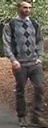
\includegraphics[height=\reidheight]{Chapters/gradrev/figures/dataset_samples/viper/a/000_45.png}&

\includegraphics[height=\reidheight]{Chapters/gradrev/figures/dataset_samples/viper/b/000_45.png}&
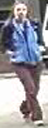
\includegraphics[height=\reidheight]{Chapters/gradrev/figures/dataset_samples/viper/a/001_45.png}&
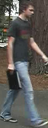
\includegraphics[height=\reidheight]{Chapters/gradrev/figures/dataset_samples/viper/b/002_90.png}&
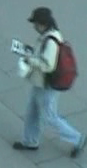
\includegraphics[height=\reidheight]{Chapters/gradrev/figures/dataset_samples/PRID/a/img_0001.png}&
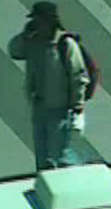
\includegraphics[height=\reidheight]{Chapters/gradrev/figures/dataset_samples/PRID/b/img_0001.png}&
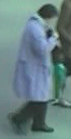
\includegraphics[height=\reidheight]{Chapters/gradrev/figures/dataset_samples/PRID/a/img_0002.png}&
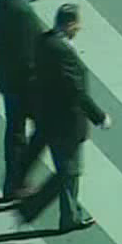
\includegraphics[height=\reidheight]{Chapters/gradrev/figures/dataset_samples/PRID/b/img_0003.png}&
\includegraphics[height=\reidheight]{Chapters/gradrev/figures/dataset_samples/cuhk/a/001_00005.png}&
\includegraphics[height=\reidheight]{Chapters/gradrev/figures/dataset_samples/cuhk/b/001_00221.png}&
\includegraphics[height=\reidheight]{Chapters/gradrev/figures/dataset_samples/cuhk/a/002_00280.png}&
\includegraphics[height=\reidheight]{Chapters/gradrev/figures/dataset_samples/cuhk/b/003_00403.png}\\
\multicolumn{4}{c}{VIPER}&
\multicolumn{4}{c}{PRID}&
\multicolumn{4}{c}{CUHK}
\end{tabular}
\caption{Matching and non-matching pairs of probe-gallery images from different person re-identification data sets. The three data sets are treated as different domains in our experiments.}
\label{fig:reidsamples}
\end{figure*}

\addtolength{\tabcolsep}{3pt}

Following \citet{YiLL14}, we augmented our data with mirror images, and during test time we calculate similarity score between two images as the mean of the four scores corresponding to different flips of the two compared images. In case of CUHK, where there are 4 images (including mirror images) for each of the two camera views for each person, all 16 combinations' scores are averaged. 

\subsubsection{CNN architectures and Training Procedure} 

In our experiments, we use siamese architecture described in \citet{YiLL14} (\textit{Deep Metric Learning} or \textit{DML}) for learning deep image descriptors on the source data set.
This architecture incorporates two convolution layers (with $7\times7$ and $5\times5$ filter banks), followed by ReLU and max pooling, and one fully-connected layer, which gives $500$-dimensional descriptors as an output. There are three parallel flows within the CNN for processing three part of an image: the upper, the middle, and the lower one. The first convolution layer shares parameters between three parts, and the outputs of the second convolution layers are concatenated.
During training, we follow \citet{YiLL14} and calculate pairwise cosine similarities between $500$-dimensional features within each batch and backpropagate the loss for all pairs within batch. 

To perform domain-adversarial training, we construct a DANN architecture.  The feature extractor includes the two convolutional layers (followed by max-pooling and ReLU) discussed above. The label predictor in this case is replaced with \textit{descriptor predictor} that includes one fully-connected layer. The domain classifier includes two fully-connected layers with $500$ units in the intermediate representation ($x{\rightarrow}500{\rightarrow}1$). 

For the verification loss function in the descriptor predictor we used Binomial Deviance loss, defined in \citet{YiLL14} with similar parameters: $\alpha = 2$, $\beta = 0.5$, $c = 2$ (the asymmetric cost parameter for negative pairs). The domain classifier is trained with logistic loss as in subsection  \ref{train_proc_for_classification}.

We used learning rate fixed to $0.001$ and momentum of $0.9$. The schedule of adaptation similar to the one described in subsection \ref{train_proc_for_classification} was used. We also inserted dropout layer with rate $0.5$ after the concatenation of outputs of the second max-pooling layer. $128$-sized batches were used for source data and $128$-sized batches for target data. 

%TODO fix 
% \begin{figure*}[t]
%   \definecolor{fnodebottom}{RGB}{132,170,81}
%   \definecolor{fnodetop}{RGB}{172,222,106}
%   \definecolor{cnodebottom}{RGB}{120,128,164}
%   \definecolor{cnodetop}{RGB}{158,167,218}
%   \definecolor{dnodebottom}{RGB}{174,109,146}
%   \definecolor{dnodetop}{RGB}{230,141,192}
%   \centering
%   {%
%      \scalebox{0.65}{\input{./Chapters/gradrev/figures/archs/reidentification_adaptation.tikz}}}\\
%   \caption{CNN architecture used in experiments on domain adaptation for person re-identification}
%   \label{fig:reid_arch}
% \end{figure*}

\subsubsection{Results on Re-identification data sets} 

\begin{figure}[t]
\centering
  \begin{tabular}{p{5cm}  p{5cm}  p{5cm} }
      
        \setlength\figureheight{3.5cm}
        \setlength\figurewidth{3.5cm}
        \begin{tikzpicture}[font=\scriptsize]

\begin{axis}[%
width=0.95092\figurewidth,
height=\figureheight,
at={(0\figurewidth,0\figureheight)},
scale only axis,
xmin=1,
xmax=50,
xlabel={Rank},
ymin=0,
ymax=1,
ylabel={Identification rate (\%)},
axis x line*=bottom,
axis y line*=left,
legend style={at={($ (0,1) + (+0.1cm,+0.1cm) $)},anchor=north west,align=left,legend cell align=left,draw=black},
xmajorgrids,
ymajorgrids,
grid style={dashed}
]
\addplot [color=blue,solid,line width=1.0pt]
  table[row sep=crcr]{%
1    0.1518987341772152\\
5    0.34810126582278483\\
10   0.47468354430379744\\
15   0.5474683544303798\\
20   0.5886075949367089\\
25   0.629746835443038\\
30   0.6613924050632911\\
35   0.680379746835443\\
40   0.7120253164556962\\
45   0.7183544303797469\\
50   0.7310126582278481\\
};
\addlegendentry{DML};

\addplot [color=cyan,solid,line width=1.0pt]
  table[row sep=crcr]{%
1    0.14556962025316456\\
5    0.3322784810126582\\
10   0.4873417721518987\\
15   0.5569620253164557\\
20   0.5917721518987342\\
25   0.6424050632911392\\
30   0.689873417721519\\
35   0.7025316455696202\\
40   0.7278481012658228\\
45   0.7531645569620253\\
50   0.7848101265822784\\
};
\addlegendentry{DML, adaptation};



\end{axis}
\end{tikzpicture}%
        \centering\small{(a) Whole CUHK $\rightarrow$ VIPeR}
        \label{fig:allcuhk_viper}
  
    &
        \setlength\figureheight{3.5cm}
        \setlength\figurewidth{3.5cm}
        \begin{tikzpicture}[font=\scriptsize]

\begin{axis}[%
width=0.95092\figurewidth,
height=\figureheight,
at={(0\figurewidth,0\figureheight)},
scale only axis,
xmin=1,
xmax=50,
xlabel={Rank},
ymin=0,
ymax=1,
ylabel={Identification rate (\%)},
axis x line*=bottom,
axis y line*=left,
legend style={at={($ (0,1) + (+0.1cm,+0.1cm) $)},anchor=north west,align=left,legend cell align=left,draw=black},
xmajorgrids,
ymajorgrids,
grid style={dashed}
]
\addplot [color=blue,solid,line width=1.0pt]
  table[row sep=crcr]{%
1      0.126582278481 \\
5      0.303797468354 \\
10      0.414556962025 \\
15      0.490506329114 \\
20      0.550632911392 \\
25      0.613924050633 \\
30      0.651898734177 \\
35      0.686708860759 \\
40      0.708860759494 \\
45      0.75 \\
50      0.759493670886 \\
};
\addlegendentry{DML};

\addplot [color=cyan,solid,line width=1.0pt]
  table[row sep=crcr]{%
1      0.120253164557 \\
5      0.29746835443 \\
10      0.462025316456 \\
15      0.541139240506 \\
20      0.594936708861 \\
25      0.617088607595 \\
30      0.645569620253 \\
35      0.667721518987 \\
40      0.696202531646 \\
45      0.712025316456 \\
50      0.73417721519 \\
};
\addlegendentry{DML, adaptation};


\end{axis}
\end{tikzpicture}%
        \centering\small{(b) CUHK/p1 $\rightarrow$ VIPeR}
%        \label{fig:cuhk_p1_viper}
    &
        \setlength\figureheight{3.5cm}
        \setlength\figurewidth{3.5cm}
        \begin{tikzpicture}[font=\scriptsize]

\begin{axis}[%
width=0.95092\figurewidth,
height=\figureheight,
at={(0\figurewidth,0\figureheight)},
scale only axis,
xmin=1,
xmax=50,
xlabel={Rank},
ymin=0,
ymax=1,
ylabel={Identification rate (\%)},
axis x line*=bottom,
axis y line*=left,
legend style={at={($ (0,1) + (+0.1cm,+0.1cm) $)},anchor=north west,align=left,legend cell align=left,draw=black},
xmajorgrids,
ymajorgrids,
grid style={dashed}
]
\addplot [color=blue,solid,line width=1.0pt]
  table[row sep=crcr]{%
1      0.0664556962025 \\
5      0.167721518987 \\
10      0.253164556962 \\
15      0.275316455696 \\
20      0.316455696203 \\
25      0.348101265823 \\
30      0.379746835443 \\
35      0.414556962025 \\
40      0.45253164557 \\
45      0.474683544304 \\
50      0.496835443038 \\
};
\addlegendentry{DML};

\addplot [color=cyan,solid,line width=1.0pt]
  table[row sep=crcr]{%
1      0.0632911392405 \\
5      0.161392405063 \\
10      0.259493670886 \\
15      0.338607594937 \\
20      0.389240506329 \\
25      0.417721518987 \\
30      0.439873417722 \\
35      0.471518987342 \\
40      0.496835443038 \\
45      0.518987341772 \\
50      0.53164556962 \\
};
\addlegendentry{DML, adaptation};


\end{axis}
\end{tikzpicture}%
        \centering\small{(c) PRID $\rightarrow$ VIPeR}
%        \label{fig:cuhk_p1_viper} \\    
 \end{tabular}
%  \caption{Results on VIPeR}
%  \label{fig:viper}
% \end{figure}%

% \begin{figure}[h]
% \centering
 \begin{tabular}{ p{5cm}  p{5cm}  p{5cm} }
        \setlength\figureheight{3.5cm}
        \setlength\figurewidth{4cm}
        \begin{tikzpicture}[font=\scriptsize]

\begin{axis}[%
width=0.95092\figurewidth,
height=\figureheight,
at={(0\figurewidth,0\figureheight)},
scale only axis,
xmin=1,
xmax=50,
xlabel={Rank},
ymin=0,
ymax=1,
ylabel={Identification rate (\%)},
axis x line*=bottom,
axis y line*=left,
legend style={at={($ (0,1) + (+0.1cm,+0.1cm) $)},anchor=north west,align=left,legend cell align=left,draw=black},
xmajorgrids,
ymajorgrids,
grid style={dashed}
]
\addplot [color=blue,solid,line width=1.0pt]
  table[row sep=crcr]{%
1    0.08\\
5    0.13\\
10   0.22\\
15   0.27\\
20   0.31\\
25   0.35\\
30   0.4\\
35   0.41\\
40   0.41\\
45   0.43\\
50   0.44\\
};
\addlegendentry{DML};

\addplot [color=cyan,solid,line width=1.0pt]
  table[row sep=crcr]{%
1    0.07\\
5    0.19\\
10   0.27\\
15   0.32\\
20   0.35\\
25   0.37\\
30   0.39\\
35   0.41\\
40   0.43\\
45   0.45\\
50   0.45\\
};
\addlegendentry{DML, adaptation};


%[0.08, 0.13, 0.22, 0.27, 0.31, 0.35, 0.4, 0.41, 0.41, 0.43, 0.44]
%[0.07, 0.19, 0.27, 0.32, 0.35, 0.37, 0.39, 0.41, 0.43, 0.45, 0.45]

%
\end{axis}
\end{tikzpicture}%





        \centering\small{(d) Whole CUHK $\rightarrow$ PRID}
        \label{fig:allcuhk_prid}
    &
        \setlength\figureheight{3.5cm}
        \setlength\figurewidth{4cm}
        \begin{tikzpicture}[font=\scriptsize]

\begin{axis}[%
width=0.95092\figurewidth,
height=\figureheight,
at={(0\figurewidth,0\figureheight)},
scale only axis,
xmin=1,
xmax=50,
xlabel={Rank},
ymin=0,
ymax=1,
ylabel={Identification rate (\%)},
axis x line*=bottom,
axis y line*=left,
legend style={at={($ (0,1) + (+0.1cm,+0.1cm) $)},anchor=north west,align=left,legend cell align=left,draw=black},
xmajorgrids,
ymajorgrids,
grid style={dashed}
]
\addplot [color=blue,solid,line width=1.0pt]
  table[row sep=crcr]{%
1      0.04 \\
5      0.08 \\
10      0.15 \\
15      0.22 \\
20      0.25 \\
25      0.3 \\
30      0.32 \\
35      0.36 \\
40      0.39 \\
45      0.41 \\
50      0.44 \\
};
\addlegendentry{DML};

\addplot [color=cyan,solid,line width=1.0pt]
  table[row sep=crcr]{%
1      0.06 \\
5      0.16 \\
10      0.21 \\
15      0.27 \\
20      0.31 \\
25      0.36 \\
30      0.39 \\
35      0.41 \\
40      0.41 \\
45      0.42 \\
50      0.43 \\
};
\addlegendentry{DML, adaptation};


\end{axis}
\end{tikzpicture}%
        \centering\small{(e) CUHK/p1 $\rightarrow$ PRID}
        \label{fig:cuhk_p1_prid}
    &
       \setlength\figureheight{3.5cm}
       \setlength\figurewidth{4cm}
       \begin{tikzpicture}[font=\scriptsize]

\begin{axis}[%
width=0.95092\figurewidth,
height=\figureheight,
at={(0\figurewidth,0\figureheight)},
scale only axis,
xmin=1,
xmax=50,
xlabel={Rank},
ymin=0,
ymax=1,
ylabel={Identification rate (\%)},
axis x line*=bottom,
axis y line*=left,
legend style={at={($ (0,1) + (+0.1cm,+0.1cm) $)},anchor=north west,align=left,legend cell align=left,draw=black},
xmajorgrids,
ymajorgrids,
grid style={dashed}
]
\addplot [color=blue,solid,line width=1.0pt]
  table[row sep=crcr]{%
1      0.08 \\
5      0.15 \\
10      0.19 \\
15      0.25 \\
20      0.28 \\
25      0.34 \\
30      0.35 \\
35      0.36 \\
40      0.39 \\
45      0.4 \\
50      0.41 \\
};
\addlegendentry{DML};

\addplot [color=cyan,solid,line width=1.0pt]
  table[row sep=crcr]{%
1      0.07 \\
5      0.19 \\
10      0.25 \\
15      0.27 \\
20      0.31 \\
25      0.36 \\
30      0.39 \\
35      0.42 \\
40      0.42 \\
45      0.46 \\
50      0.47 \\
};
\addlegendentry{DML, adaptation};


\end{axis}
\end{tikzpicture}%
        \centering\small{(f) VIPeR $\rightarrow$ PRID}
        \label{fig:viper_prid}  \\    
 \end{tabular}
%  \caption{Results on PRID}
%  \label{fig:prid}
% \end{figure}


% \begin{figure}[h]
% \centering
 \begin{tabular}{ p{5cm}  p{5cm}}
        \setlength\figureheight{3.5cm}
        \setlength\figurewidth{4cm}
        \begin{tikzpicture}[font=\scriptsize]

\begin{axis}[%
width=0.95092\figurewidth,
height=\figureheight,
at={(0\figurewidth,0\figureheight)},
scale only axis,
xmin=1,
xmax=50,
xlabel={Rank},
ymin=0,
ymax=1,
ylabel={Identification rate (\%)},
axis x line*=bottom,
axis y line*=left,
legend style={at={($ (0,1) + (+0.1cm,+0.1cm) $)},anchor=north west,align=left,legend cell align=left,draw=black},
xmajorgrids,
ymajorgrids,
grid style={dashed}
]
\addplot [color=blue,solid,line width=1.0pt]
  table[row sep=crcr]{%
1      0.109053497942 \\
5      0.265432098765 \\
10      0.366255144033 \\
15      0.407407407407 \\
20      0.465020576132 \\
25      0.491769547325 \\
30      0.510288065844 \\
35      0.541152263374 \\
40      0.572016460905 \\
45      0.59670781893 \\
50      0.617283950617 \\
};
\addlegendentry{DML};

\addplot [color=cyan,solid,line width=1.0pt]
  table[row sep=crcr]{%
1      0.125514403292 \\
5      0.253086419753 \\
10      0.366255144033 \\
15      0.440329218107 \\
20      0.5 \\
25      0.5329218107 \\
30      0.572016460905 \\
35      0.594650205761 \\
40      0.617283950617 \\
45      0.650205761317 \\
50      0.668724279835 \\
};
\addlegendentry{DML, adaptation};


\end{axis}
\end{tikzpicture}%
        \centering\small{(g) VIPeR $\rightarrow$ CUHK/p1}
        \label{fig:viper_cuhk_p1}
    &
        \setlength\figureheight{3.5cm}
        \setlength\figurewidth{4cm}
        \begin{tikzpicture}[font=\scriptsize]

\begin{axis}[%
width=0.95092\figurewidth,
height=\figureheight,
at={(0\figurewidth,0\figureheight)},
scale only axis,
xmin=1,
xmax=50,
xlabel={Rank},
ymin=0,
ymax=1,
ylabel={Identification rate (\%)},
axis x line*=bottom,
axis y line*=left,
legend style={at={($ (0,1) + (+0.1cm,+0.1cm) $)},anchor=north west,align=left,legend cell align=left,draw=black},
xmajorgrids,
ymajorgrids,
grid style={dashed}
]
\addplot [color=blue,solid,line width=1.0pt]
  table[row sep=crcr]{%
1      0.0569620253165 \\
5      0.139240506329 \\
10      0.212025316456 \\
15      0.284810126582 \\
20      0.316455696203 \\
25      0.344936708861 \\
30      0.370253164557 \\
35      0.389240506329 \\
40      0.414556962025 \\
45      0.443037974684 \\
50      0.465189873418 \\
};
\addlegendentry{DML};

\addplot [color=cyan,solid,line width=1.0pt]
  table[row sep=crcr]{%
1      0.0843621399177 \\
5      0.191358024691 \\
10      0.263374485597 \\
15      0.316872427984 \\
20      0.347736625514 \\
25      0.395061728395 \\
30      0.432098765432 \\
35      0.471193415638 \\
40      0.504115226337 \\
45      0.5329218107 \\
50      0.553497942387 \\
};
\addlegendentry{DML, adaptation};


\end{axis}
\end{tikzpicture}%
        \centering\small{(h) PRID $\rightarrow$ CUHK/p1}
        \label{fig:prid_cuhk_p1}
  \\    
  \end{tabular}
  \caption{Results on VIPeR, PRID and CUHK/p1 with and without domain-adversarial learning. Across the eight domain pairs domain-adversarial learning improves re-identification accuracy. For some domain pairs the improvement is considerable.}
  \label{fig:adaptresults}
\end{figure}

Figure \ref{fig:adaptresults} shows results in the form of CMC-curves for eight pairs of data sets. Depending on the hardness of the annotation problem we trained either for 50,000 iterations (CUHK/p1 $\rightarrow$ VIPeR, VIPeR $\rightarrow$ CUHK/p1, PRID $\rightarrow$ VIPeR) or for 20,000 iterations (the other five pairs). 

\begin{figure*}
\centering
\begin{tabular}{c c}
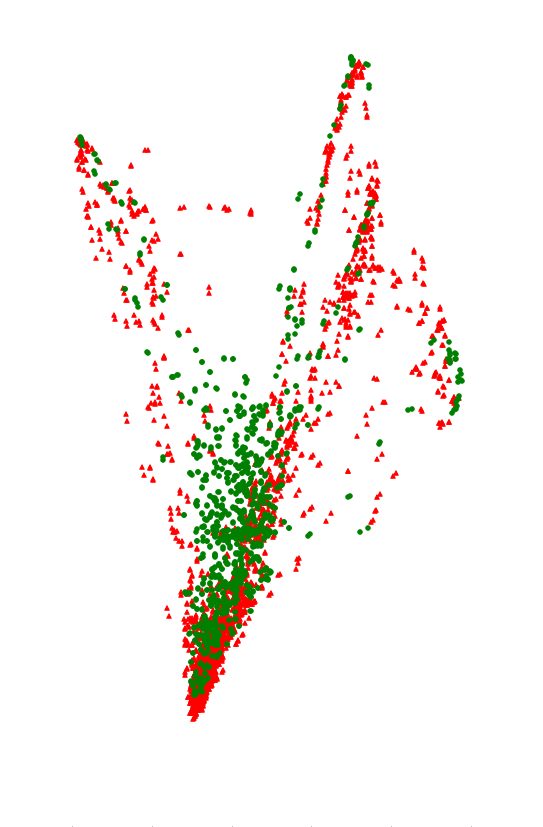
\includegraphics[height=7cm, width=7cm]{./Chapters/gradrev/figures/reid_adapt_results/viper_cuhkp1_zc.png}&
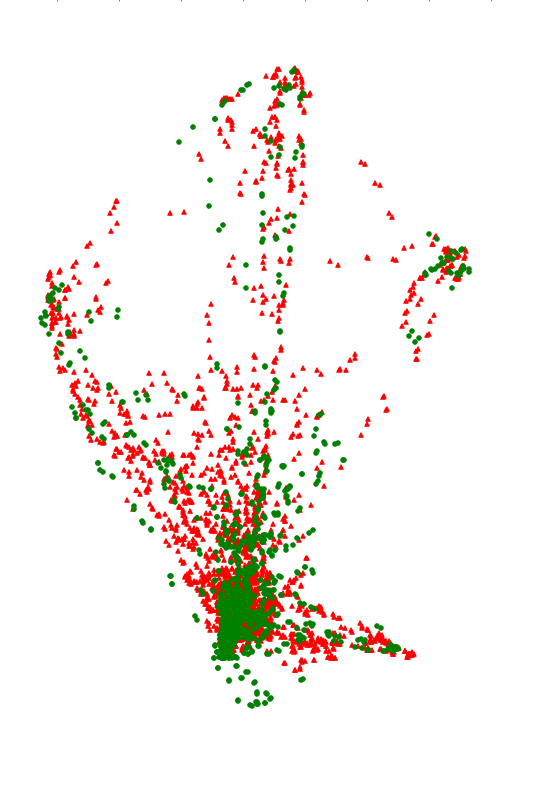
\includegraphics[height=7cm, width=7cm]{./Chapters/gradrev/figures/reid_adapt_results/viper_cuhkp1_da.png}\\
\small{(a) DML}&
\small{(b) DML, adaptation}\\
\end{tabular}
\caption{The effect of adaptation shown by t-SNE visualizations of source and target domains descriptors in a VIPeR $\rightarrow$ CUHK/p1 experiment pair. VIPeR is depicted with \textit{green} and CUHK/p1 - with \textit{red}. As in the image classification case, domain-adversarial learning ensures a closer match between the source and the target distributions. }
\label{fig:reidtsne}
\end{figure*}


After the sufficient number of iterations, domain-adversarial training consistently improves the performance of re-identification. For the pairs that involve PRID data set, which is more dissimilar to the other two data sets, the improvement is considerable. Overall, this demonstrates the applicability of the domain-adversarial learning beyond classification problems.

Figure \ref{fig:reidtsne} further demonstrates the effect of adaptation on the distributions of the learned descriptors in the source and in target sets in VIPeR $\rightarrow$ CUHK/p1 experiments, where domain adversarial learning once again achieves better intermixing of the two domains.


\section{Conclusion}

The paper proposes a new approach to domain adaptation of feed-forward neural networks, which allows large-scale training based on large amount of annotated data in the source domain and large amount of unannotated data in the target domain. Similarly to many previous shallow and deep DA techniques, the adaptation is achieved through aligning the distributions of features across the two domains. However, unlike previous approaches, the alignment is accomplished through standard backpropagation training.

The approach is motivated and supported by the domain adaptation theory of \citet{BenDavid-NIPS06,BenDavid-MLJ2010}. 
The main idea behind DANN is to enjoin the network hidden layer to learn a representation which is predictive of the source example labels, but uninformative about the domain of the input (source or target). 
We implement this new approach within both shallow and deep feed-forward architectures. The latter allows simple implementation within virtually any deep learning package through the introduction of a simple gradient reversal layer. 
We have shown that our approach is flexible and achieves state-of-the-art results on a variety of benchmark in domain adaptation, namely for sentiment analysis and image classification tasks. 

A convenient aspect of our approach is that the domain adaptation component can be added to almost any neural network architecture that is trainable with backpropagation. Towards this end, We have demonstrated experimentally that the approach is not confined to classification tasks but can be used in other feed-forward architectures, e.g.\ for descriptor learning for person re-identification.


\section{Motivation}




%problem intuition
In many practical cases, we do not have access to a sufficient amount of labeled training data for supervised learning. This problem is especially critical for learning deep neural networks that often incorporate millions of parameters. However, it is often the case that the training data are available, and the labeling corresponds to the task of interest, but the data differ from those that our predictor will encounter during test time. Such difference between the training data (source) and possible test data (target) is referred to as a \textit{domain shift} or \textit{covariate shift}. In more detail, this means that the source and target data share the same feature space, and only their marginal distributions are assumed to be different. 

%example
One important example of the described situation is training on synthetic images that can be generated automatically (\eg{} by 3D rendering systems). This is a particularly practical use case, as collecting the necessary amount of analogous real data and its labeling may be very time-consuming. 
In this way, the ability to overcome the domain shift between the available synthetic and target data is crucial for the final performance of the predictor. 

%notation?

%how others solve the problem
Although there exist many powerful methods for domain adaptation \cite{huang2007correcting, pan2008transfer, pan2011domain,baktashmotlagh2013unsupervised,gong2012geodesic,gong2013connecting}, they most often work for the fixed feature representations and therefore are limited by these representations. %Most often, such methods cannot be naturally incorporated to the process of learning deep neural network. 

Several works have also approached domain adaptation in the framework of deep learning. \cite{glorot2011domain} and \cite{chopra2013dlid} train the denoising autoencoders on a mixture of data from the two domains to get the domain-invariant feature extractors. The task-specific training is performed as the second step (although, at this step, \cite{chopra2013dlid} finetunes both task-specific neural network and the pre-trained feature extractor using the task-specific loss). In contrast to \cite{glorot2011domain} and \cite{chopra2013dlid}, \cite{LongC0J15} and \cite{tzeng2014deep} apply a special loss function (based on Maximum Mean Discrepancy) to pull the two domains closer. Such an objective can be optimized simultaneously with the task-specific loss. This allows to learn the representations that are useful for the task of interest and at the same time are domain-invariant.

%how it is suggested in the paper
A new way of deep domain adaptation is suggested in this chapter. Like in the works of \cite{LongC0J15} and \cite{tzeng2014deep}, the goal is to incorporate domain adaptation into the process of training a classification neural network, so that the learned deep representations are 
\begin{itemize}
    \item discriminative (\ie{} useful for classification),
    \item  domain-invariant (\ie{} the feature distributions are close for the two domains)
\end{itemize}. 
 This is achieved by jointly optimizing the two deep discriminative classifiers:  \begin{itemize}
     \item the task-specific label predictor,
     \item the domain classifier that discriminates between the source and the target domains.
 \end{itemize}
The parameters of these two classifiers are optimized in order to minimize their error on the training set. What provides discriminativeness and domain-invariance of the learned features is that these features are optimized simultaneously to 
\begin{itemize} 
    \item minimize the error of the task-specific classifier, 
    \item maximize the error of the domain classifier. 
 \end{itemize}

Such combination of objectives can be optimized for feed-forward networks using standard backpropagation algorithm based on stochastic gradient descent. To perform a domain-adversarial training of feature representation, the gradient reversal layer is introduced. No labeling is needed for the target domain, so the approach is suitable for \textit{unsupervised domain adaptation}.

It should be noted that an idea related to ours is described in \citep{Goodfellow14}. While their goal is quite different (building generative deep networks that can synthesize samples), the way they measure and minimize the discrepancy between the distribution of the training data and the distribution of the synthesized data is very similar to the way our architecture measures and minimizes the discrepancy between feature distributions for the two domains. %Moreover, the authors mention the problem  of saturating sigmoids which may arise at the early stages of training due to the significant dissimilarity of the domains. The technique they use to circumvent this issue (the ``adversarial'' part of the gradient is replaced by a gradient computed with respect to a suitable cost) is directly applicable to our method. 

First, the described approach is evaluated for an image classification task. This chapter includes the results only for digit classification (on the MNIST dataset \citep{LeCun98}). The extensive evaluation for many other classifications tasks can be found in the corresponding publication [\cite{ganin2016domain}].

Domain-adversarial training is also demonstrated to be applicable to person re-identification. Several publicly available datasets are considered as different domains. 
To adapt the described approach to person re-identification, we consider a \textit{descriptor predictor} trained with a Siamese-like loss instead of the label predictor trained with a classification loss. In a series of experiments, we demonstrate that domain-adversarial learning can improve cross-dataset re-identification considerably. 




%mention goodfellow, CycleGAN, about the assumption of having to adapt last layers.


\section{Domain Adaptation}
\label{section:DA_theory}

We consider classification tasks where $\Xcal$ is the input space and $\Ycal=\{0,1,\ldots,L{-}1\}$ is the set of $L$ possible labels.
Moreover, we have two different distributions over $\Xcal\!\times\! \Ycal$, called the {\it source domain} $\DS$ and the {\it target domain} $\DT$.
An \emph{unsupervised domain adaptation} learning algorithm is then provided with a {\it labeled source sample} $S$ drawn {\it i.i.d.} from $\DS$, and an {\it unlabeled target sample} $T$ drawn {\it i.i.d.} from $\DTX$, where $\DTX$ is the marginal distribution of $\DT$ over~$\Xcal$.
%\footnote{For simplicity, we consider through this paper that the source sample $S$ and the target sample $T$ are of equal size~$m$. It is easy to generalize the results for the case where $|S|\neq|T|$.}
\begin{equation*}
S = \{(\xb_i,\ys_i)\}_{i=1}^{n} \sim (\DS)^n 
\,; \quad
%\quad\mbox{and}\quad
T = \{\xb_i\}_{i=n+1}^{N} \sim (\DTX)^{n'},
\end{equation*}
with $N=n+n'$ being the total number of samples. 
%
The goal of the learning algorithm is to build a classifier $\eta:\Xcal\to\Ycal$ with a low \emph{target~risk}
\begin{equation*}
\RDT(\eta) \ \eqdef \Pr_{(\xb,\yt) \sim \DT} \Big(\eta(\xb) \neq \yt\Big)\,,
\end{equation*}
while having no information about the labels of $\DT$.

% \bigskip
% \indent\textbf{Domain Divergence}
% %\subsection{Domain Divergence}

% To tackle the challenging domain adaptation task, many  approaches bound the target error by the sum of the source error and a notion of distance between the source and the target distributions. These methods are intuitively justified by a simple assumption: the source risk is expected to be a good indicator of the target risk when both distributions are similar. Several notions of distance have been proposed for domain adaptation~\citep{BenDavid-NIPS06,Mansour-COLT09,MansourMR09,pbda}.
% In this paper, we focus on the $\Hcal$-divergence used by ~\citet{BenDavid-NIPS06}, and based on the earlier work of~\citet{kifer-2004}. Note that we assume in definition~\ref{def:Hdiv} below that the hypothesis class $\Hcal$ is a (discrete or continuous) set of binary classifiers $\eta:\Xcal\to\{0,1\}$.\footnote{As mentioned by \citet{BenDavid-NIPS06}, the same analysis holds for multiclass setting. However, to obtain the same results when $|Y|>2$, one should assume that $\Hcal$ is a symmetrical hypothesis class. That is, for all $h\in\Hcal$ and any permutation of labels $c:Y\to Y$, we have $c(h)\in \Hcal$. Note that this is the case for most commonly used neural network architectures.}
% \begin{definition}[\citealp{BenDavid-NIPS06, kifer-2004}] \label{def:Hdiv}
% Given two domain distributions $\DSX$ and $\DTX$ over~$\Xcal$, and a hypothesis class~$\Hcal$, the \emph{$\Hcal$-divergence} between $\DSX$ and $\DTX$ is
% \begin{eqnarray*}
% d_\Hcal(\DSX,\DTX)  &\eqdef & 
% 2 \,\sup_{\eta\in\Hcal} \,\bigg|\, 
% \Pr_{\xb \sim \DSX} \big[\eta(\xb) = 1\big] - 
% \Pr_{\xb \sim \DTX} \big[\eta(\xb) = 1\big]\,
% \bigg|\,.
% \end{eqnarray*}
% \end{definition}

% That is, the $\Hcal$-divergence relies on the capacity of the hypothesis class $\Hcal$ to distinguish between examples generated by $\DSX$ from examples generated by $\DTX$.
% \citet{BenDavid-NIPS06} proved that, for a symmetric hypothesis class $\Hcal$, one can compute the \emph{empirical $\Hcal$-divergence} between two samples $S\sim(\DSX)^n$ and  $T\sim(\DTX)^{n'}$ by computing
% \begin{eqnarray} \label{eq:Hdiv_empirique}
%  \hat{d}_\Hcal(S,T) & \eqdef & 
%  2\,\Bigg( 1 - \min_{\eta\in\Hcal} \bigg[
% \frac{1}{n} \sum_{i=1}^n I[\eta(\xb_i)\!=\!0] + \frac{1}{n'} \sum_{i=n+1}^{N} I[\eta(\xb_i)\!=\!1]
% \bigg] \Bigg)\,,
% \end{eqnarray}
% where $I[a]$ is the indicator function which is $1$ if predicate $a$ is true, and $0$ otherwise.

% \bigskip
% \indent\textbf{Proxy Distance}
% %\subsection{Proxy Distance}
% \label{section:PAD}

% %\citet{BenDavid-NIPS06,BenDavid-MLJ2010}
% \citet{BenDavid-NIPS06}
% suggested that, even if it is generally hard to compute $\hat{d}_\Hcal(S,T)$ exactly (\eg, when $\Hcal$ is the space of linear classifiers on $\Xcal$), we can easily approximate it by running a learning algorithm on the problem of discriminating between source and target examples. To do so, we construct a new dataset
% \begin{equation}\label{eq:U}
% U \ =\ \{(\xb_i, 0)\}_{i=1}^n \cup \{(\xb_i, 1)\}_{i=n+1}^{N}\,,
% \end{equation}
% where the examples of the source sample are labeled $0$ and the examples of the target sample are labeled $1$. Then, the risk of the classifier trained on the new dataset $U$ approximates the ``$\min$'' part of Equation~\eqref{eq:Hdiv_empirique}. 
% Given a generalization error~$\epsilon$ on the problem of discriminating between source and target examples, the $\Hcal$-divergence is then approximated by
% \begin{equation} \label{eq:PAD}
% \hat{d}_\Acal \ = \ 2\,(1-2\epsilon)\,.
% \end{equation}
% In \citep{BenDavid-NIPS06}, the value $\hat{d}_\Acal$ is called the \emph{Proxy $\Acal$-distance} (PAD). The \emph{$\Acal$-distance}
% being defined as 
% $
% d_\Acal(\DSX,\DTX)  \eqdef 
% 2 \,\sup_{A\in\Acal} \,\big|\, 
% \Pr_{\DSX} (A) - 
% \Pr_{\DTX} (A)\,
% \big|
% $,
% where $\Acal$ is a subset of $\Xcal$. Note that, by choosing $\Acal = \{A_\eta | \eta \in \Hcal\}$, with $A_\eta$ the set represented by the characteristic function $\eta$, the $\Acal$-distance and the $\Hcal$-divergence of Definition~\ref{def:Hdiv} are identical.

% In the classification experiments section of this chapter, we compute the PAD value following the approach of \citep{glorot2011domain}, \ie, we train either a linear SVM or a deeper MLP classifier on a subset of $U$ (Equation~\ref{eq:U}), and we use the obtained classifier error on the other subset as the value of~$\epsilon$ in Equation~\eqref{eq:PAD}. 
% %More details and illustrations of the linear SVM case are provided in Section~\ref{section:PAD_experiments}.

% \bigskip
% \indent\textbf{Generalization Bound on the Target Risk}

% %\subsection{Generalization Bound on the Target Risk}
% The work of \citet{BenDavid-NIPS06} also showed that the $\Hcal$-divergence $d_\Hcal(\DSX,\DTX)$ is upper bounded by its empirical estimate $\hat{d}_\Hcal(S,T)$ plus a constant complexity term that depends on the \emph{VC dimension} of $\Hcal$ and the size of samples $S$ and $T$. By combining this result with a similar bound on the source risk, the following theorem is obtained.
% \begin{theorem}[\citealp{BenDavid-NIPS06}] 
% \label{thm:RDT_bound}
% Let $\Hcal$ be a hypothesis class of VC dimension $d$.
% With probability $1-\delta$ over the choice of samples $S\sim (\DS)^n$ and $T\sim (\DTX)^{n}$, for every $\eta\in\Hcal$:
% \begin{eqnarray*}
% \RDT(\eta) &\leq&  
% \RS(\eta) +  \sqrt{\frac{4}{n}\left( d \log\tfrac{2e\, n}{d}+  \log\tfrac{4}{\delta}\right) } 
% +\hat{d}_\Hcal(S,T) + 4\sqrt{ \frac{1}{n}\left(d \log\tfrac{2 n}{d}+  \log\tfrac{4}{\delta}\right) }
% + \beta\,,
% \end{eqnarray*}
% with $\beta \geq {\displaystyle\inf_{\eta^*\in\Hcal}} \left[ \RDS(\eta^*) + \RDT(\eta^*) \right]$\,, 
% and 
% «\begin{equation*}
% \RS(\eta) \ =\ \frac{1}{n}\dsum_{i=1}^m I\left[\eta(\xb_i) \neq \ys_i\right]
% \end{equation*}
% is the {empirical source~risk}.
% %\begin{equation*}
% %\RS(\eta) \ \eqdef \ \frac{1}{m} \sum_{(\xb,y)\in S} I[\eta(\xb) = y]\,.
% %\end{equation*}
% \end{theorem}
% The previous result tells us that $\RDT(\eta)$ can be low only when the $\beta$ term is low, \ie, only when there exists a classifier that can achieve a low risk on both distributions. It also tells us that, to find a classifier with a small $\RDT(\eta)$ in a given class of fixed VC dimension, the learning algorithm should minimize (in that class) a trade-off between the source risk $\RS(\eta)$ and the empirical $\Hcal$-divergence $\hat{d}_\Hcal(S,T)$.  
% As pointed-out by~\citet{BenDavid-NIPS06}, a strategy to control the $\Hcal$-divergence is to find a representation of the examples where both the source and the target domain are as indistinguishable as possible. Under such a representation, a hypothesis with a low source risk will, according to Theorem~\ref{thm:RDT_bound}, perform well on the target data.  
% In this paper, we present an algorithm that directly exploits this idea.


\section{Domain-Adversarial Neural Networks (DANN)}
\label{section:dann}

%An original aspect of our approach is to explicitly implement the idea exhibited by Theorem~\ref{thm:RDT_bound} 
%into a neural network classifier.
To learn a
model that can generalize well from one domain to another, we ensure that
the internal representation of the neural network contains no discriminative information about the origin of the input (source or target), while preserving a low risk on the source (labeled) examples.

In this section, we detail the proposed approach for incorporating a ``domain adaptation component'' to neural networks.
%In Subsection~\ref{section:shallow_dann}, we start by developing the idea for the simplest possible case, \ie,  a single hidden layer, fully connected neural network. We then describe how to generalize the approach to arbitrary  (deep) network architectures. 




 \begin{figure*}[t]
 \centering
 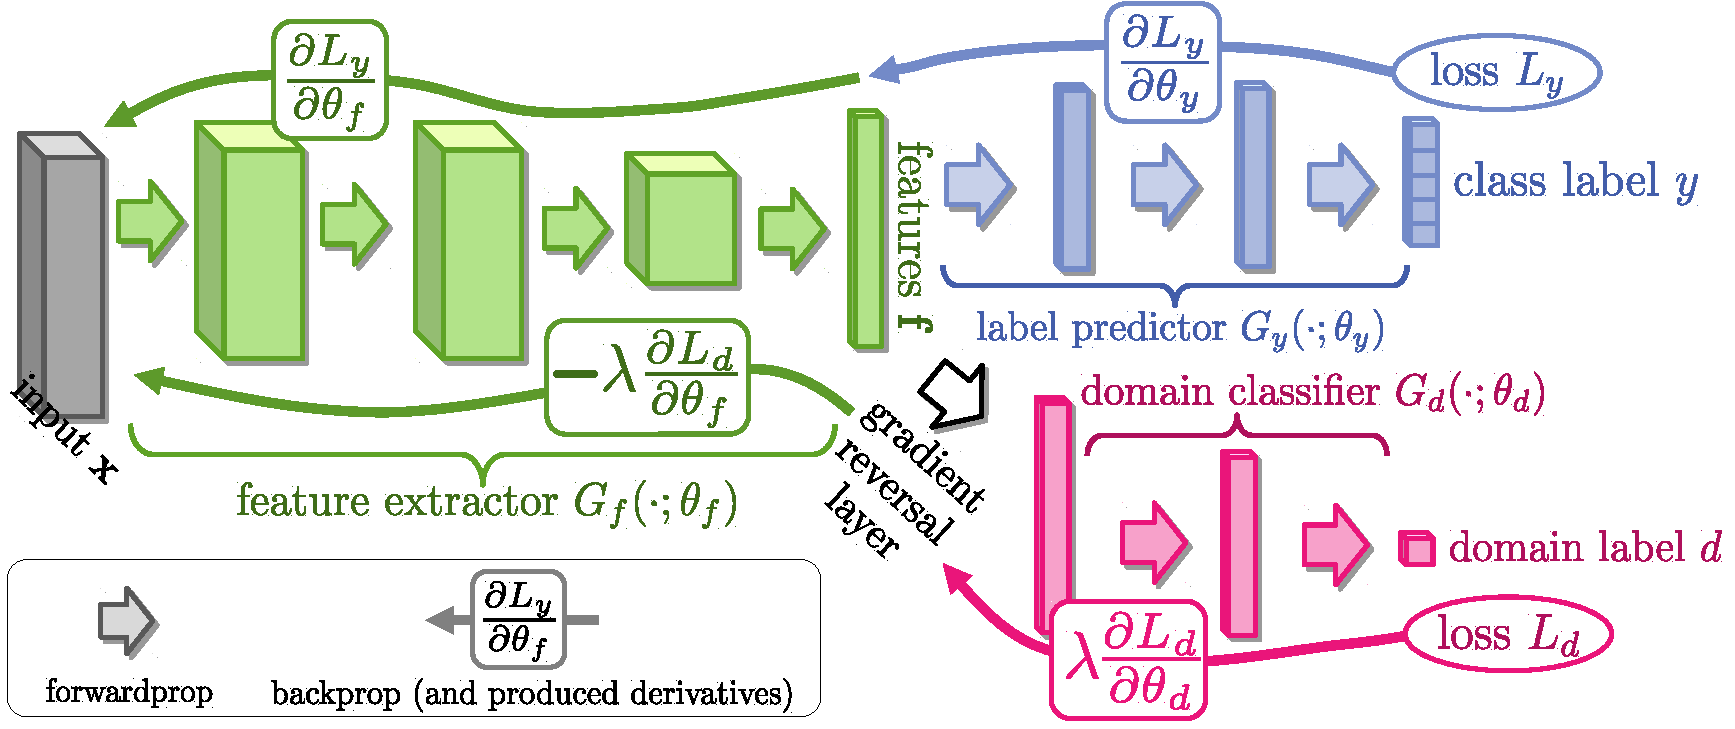
\includegraphics[width=0.85\textwidth]{Chapters/gradrev/figures/deepDA2_c.pdf}
 \caption{The {\bf proposed architecture} includes a deep {\em feature extractor} (green) and a deep {\em label predictor} (blue), which together form a standard feed-forward architecture. Unsupervised domain adaptation is achieved by adding a {\em domain classifier} (red) connected to the feature extractor via a {\em gradient reversal layer} that multiplies the gradient by a certain negative constant during the backpropagation-based training. Otherwise, the training proceeds standardly and minimizes the label prediction loss (for source examples) and the domain classification loss (for all samples). Gradient reversal ensures that the feature distributions over the two domains are made similar (as indistinguishable as possible for the domain classifier), thus resulting in the domain-invariant features.\vspace{-2mm}}
 \label{fig:arch}
 \end{figure*}
 

%\bigskip
%\indent\textbf{Generalization to Arbitrary Architectures}


%\subsection{Generalization to Arbitrary Architectures}
%\label{section:deep_DANN}
%
%We now detail the proposed model for the domain adaptation. We assume that the model works with input samples $\x \in X$, where $X$ is some input space and certain labels (output) $y$ from the label space $Y$. Below, we assume classification problems where $Y$ is a finite set ($Y=\{1,2,\dots L\}$), however our approach is generic and can handle any output label space that other deep feed-forward models can handle. We further assume that there exist two distributions $\S(x,y)$ and $\T(x,y)$ on $X\otimes Y$, which will be referred to as the source distribution and the target distribution (or the source domain and the target domain). Both distributions are assumed complex and unknown, and furthermore similar but different (in other words, $\S$ is ``shifted'' from $\T$ by some {\em domain shift}). 

%Our ultimate goal is to be able to predict labels $y$ given the input $\x$ for the target distribution. At training time, we have an access to a large set of training samples $\{\x_1,\x_2,\dots,\x_N\}$ from both the source and the target domains distributed according to the marginal distributions $\S(\x)$ and $\T(\x)$. We denote with $d_i$ the binary variable ({\em domain label}) for the $i$-th example, which indicates whether $x_i$ come from the source distribution ($\x_i{\sim}\S(\x)$ if $d_i{=}0$) or from the target distribution ($\x_i{\sim}\T(\x)$ if $d_i{=}1$). For the examples from the source distribution ($d_i{=}0$) the corresponding labels $y_i \in Y$ are known at training time. For the examples from the target domains, we do not know the labels at training time, and we want to predict such labels at test time.

For illustration purposes, we've so far focused on the case of a single hidden layer DANN. However, it is straightforward to generalize to other sophisticated architectures, which might be more appropriate for the data at hand. For example,  deep convolutional neural networks are well known for being state-of-the-art models for learning discriminative features of images~\citep{Krizhevsky12}.

Let us now use a more general notation for the different components of DANN. Namely, let $G_f(\cdot; \tf)$ be the $D$-dimensional neural network feature extractor, with parameters $\tf$. Also, let $G_y(\cdot; \ty)$ be the part of DANN that computes the network's label prediction output layer, with parameters $\ty$, while $G_d(\cdot;\td)$ now corresponds to the computation of the domain prediction output of the network, with parameters $\td$.
%Note that for preserving the theoretical guarantees of Theorem~\ref{thm:RDT_bound}, the hypothesis class $\Hcal_d$ generated by the domain prediction component $G_d$ should include the hypothesis class $\Hcal_y$ generated by the label prediction component $G_y$. Thus, $\Hcal_y\subseteq\Hcal_d$.

We will note the prediction loss and the domain loss respectively by
\begin{eqnarray*}
\Lcal_y^i(\tf, \ty)&=& \Lcal_{y} \big( G_y(G_f(\xb_i; \tf); \ty), y_i\big)\,,\\ 
\Lcal_{d}^i(\tf, \td)&=& \Lcal_{d} \big( G_d(G_f(\xb_i; \tf); \td), d_i)\,.
\end{eqnarray*}
% :)
Training DANN then consists in optimizing
\begin{eqnarray}
E (\tf,\ty,\td)
= \frac{1}{n}\sum_{i=1}^n \Lcal_y^i(\tf,\ty)
- \lambda \,\Big(\frac{1}{n} \sum_{i=1}^{n} \Lcal_{d}^i(\tf, \td)  + \frac{1}{n'} \sum_{\mathclap{i=n+1}}^{N} \Lcal_{d}^i(\tf, \td )\Big),
\label{eqn:global_gen}
\end{eqnarray}
by finding the saddle point $\htf,\hty,\htd$ such that
\begin{eqnarray}
(\htf,\hty) &=& \argmin_{\tf,\ty}\, E(\tf,\ty,\htd)\,,\label{eq:opt1}\\\label{eq:opt2}
\htd &=& \argmax_\td \, E(\htf,\hty, \td)\,.
\end{eqnarray}




As suggested previously, a saddle point defined by Equations~(\ref{eq:opt1}-\ref{eq:opt2}) can be found as a stationary point of the following gradient updates:
{\allowdisplaybreaks[4]
\begin{align}
\tf \quad &\longleftarrow \quad \tf \;-\; \mu \left(\frac{\partial \Lcal_y^i}{\partial \tf}-\lambda\frac{\partial \Lcal_d^i}{\partial \tf} \right), \label{eq:upd1}\\
\ty \quad &\longleftarrow \qquad \ty \;-\; \mu \frac{\partial \Lcal_y^i}{\partial \ty}\,,\label{eq:upd2}\\
\td \quad &\longleftarrow \qquad \td \;-\; \mu \lambda \frac{\partial \Lcal_d^i}{\partial \td}\,, \label{eq:upd3}
\end{align}
}where $\mu$ is the learning rate. We use stochastic estimates of these gradients, by sampling examples from the dataset.

The updates of Equations~(\ref{eq:upd1}-\ref{eq:upd3}) are very similar to stochastic gradient descent (SGD) updates for a feed-forward deep model that comprises feature extractor fed into the label predictor and into the domain classifier (with loss weighted by $\lambda$). The only difference is that in \eq{upd1}, the gradients from the class and domain predictors are subtracted, instead of being summed (the difference is important, as otherwise SGD would try to make features dissimilar across domains in order to minimize the domain classification loss). Since SGD, and its many variants, is the main learning algorithm implemented in most libraries for deep learning, it would be convenient to frame an implementation of our stochastic saddle point procedure as SGD.

Fortunately, such a reduction can be accomplished by introducing a special \emph{gradient reversal layer} (GRL), defined as follows. The gradient reversal layer has no parameters associated with it.
%(apart from the meta-parameter $\lambda$, which is not updated by backpropagation). 
During the forward propagation, the GRL acts as an identity transformation. During the backpropagation however, the GRL takes the gradient from the subsequent level and changes its sign, \ie multiplies it by $-1$, before passing it to the preceding layer. Implementing such a layer using existing object-oriented packages for deep learning is simple, requiring only to define procedures for the forward propagation (identity transformation), and backpropagation (multiplying by $-1$). The layer requires no parameter update. 

The GRL as defined above is inserted between the feature extractor $G_f$ and the domain classifier $G_d$, resulting in the architecture depicted in \fig{arch}. As the backpropagation process passes through the GRL, the partial derivatives of the loss that is downstream the GRL (\ie, $\Lcal_d$) w.r.t.\ the layer parameters that are upstream the GRL (\ie, $\tf$) get multiplied by $-1$, \ie, $\frac{\partial \Lcal_d}{\partial \tf}$ is effectively replaced with $-\frac{\partial \Lcal_d}{\partial \tf}$. Therefore, running SGD in the resulting model implements the updates of Equations~(\ref{eq:upd1}-\ref{eq:upd3}) and converges to a saddle point of Equation~\eqref{eqn:global_gen}.

Mathematically, we can formally treat the gradient reversal layer as a ``pseudo-function'' ${\cal R}(\x)$ defined by two (incompatible) equations describing its forward and backpropagation behaviour:
\begin{align}
{\cal R}(\x) = \x\,,\\
\frac{d{\cal R}}{d\x} = -\mathbf{I}\,,
\end{align}
where $\mathbf{I}$ is an identity matrix.
We can then define the objective ``pseudo-function'' of $(\tf,\ty,\td)$ that is being optimized by the stochastic gradient descent within our method:
\begin{eqnarray}
&&\tilde E (\tf,\ty,\td) = \! \frac{1}{n}\sum_{i=1}^n \Lcal_y\left( \strut G_y(G_f(\x_i;\tf);\ty), y_i\right)\label{eq:pseudoobj}\\
&&~~~- \lambda \,\Big(\frac{1}{n} \sum_{i=1}^{n} \Lcal_d \left( \strut G_d({\cal R}(G_f(\x_i;\tf));\td), d_i\right) + \frac{1}{n'} \sum_{\mathclap{i=n+1}}^{N} \Lcal_d \left( \strut G_d({\cal R}(G_f(\x_i;\tf));\td), d_i\right) \Big)\,.\nonumber
\end{eqnarray}

Running updates (\ref{eq:upd1}-\ref{eq:upd3}) can then be implemented as doing SGD for \eq{pseudoobj} and leads to the emergence of features that are domain-invariant and discriminative at the same time. After the learning, the label predictor $G_y(G_f(\x;\tf);\ty)$ can be used to predict labels for samples from the target domain (as well as from the source domain).


\section{Experiments}
\bigskip\indent\textbf{Experiments with deep networks on image classification}\\
%\bigskip
%\indent\textbf{Experiments with Deep Networks on Image %Classification}


\label{sect:experiments}

\begin{figure*}
  \centering
  \setlength{\tabcolsep}{0pt}
  \setlength\figurewidth{0.05\textwidth}
  \renewcommand{\example}[1]{\raisebox{-.4\height}{\includegraphics[width=\figurewidth]{Chapters/gradrev/figures/domains_examples/#1}}}
  \begin{sc}
  \begin{small}
  \begin{tabular}{r@{\hskip 0.5cm} ccc c@{\hskip 0.4cm} ccc c@{\hskip 0.4cm} ccc c@{\hskip 0.4cm} ccc}
    &
    \multicolumn{3}{c}{MNIST} & &
    % \multicolumn{3}{c}{Syn Numbers} & &
    % \multicolumn{3}{c}{SVHN} & &
    % \multicolumn{3}{c}{Syn Signs}
    \\
    
    Source &
    \example{mnist_0.png} &
    \example{mnist_1.png} &
    \example{mnist_3.png} & &
    
    % \example{syn_0.png} &
    % \example{syn_1.png} &
    % \example{syn_2.png} & &
    
    % \example{svhn_3.png} &
    % \example{svhn_4.png} &
    % \example{svhn_5.png} & &
    
    % \example{synsgn_3.png} &
    % \example{synsgn_4.png} &
    % \example{synsgn_5.png}
    \\
    
    Target &
    \example{mnisti_0.png} &
    \example{mnisti_1.png} &
    \example{mnisti_2.png} & &
    
    % \example{svhn_0.png} &
    % \example{svhn_1.png} &
    % \example{svhn_2.png} & &
    
    % \example{mnist_4.png} &
    % \example{mnist_5.png} &
    % \example{mnist_6.png} & &
    
    % \example{gtsrb_2.png} &
    % \example{gtsrb_3.png} &
    % \example{gtsrb_4.png}
    \\
    
    &
    \multicolumn{3}{c}{\rule{0pt}{0.35cm} MNIST-M} & &
    % \multicolumn{3}{c}{SVHN} & &
    % \multicolumn{3}{c}{MNIST} & &
    % \multicolumn{3}{c}{GTSRB}
    \\
  \end{tabular}
  \end{small}
  \end{sc}
  \caption{Examples of domain pairs used in the experiments. See \sect{exper_quant} for details.}
  \label{fig:exper_domains_examples}
\end{figure*}

\begin{table*}[t]
\centering
    \begin{small}
      \begin{sc}
        \renewcommand{\arraystretch}{1.3}
        \rowcolors{2}{black!10}{}
        \begin{tabular}{l r | c c c c}
          \hline
          \multirow{2}{*}{Method} & {\scriptsize Source} & MNIST \\ %& Syn Numbers & SVHN & Syn Signs \\
          & {\scriptsize Target} & MNIST-M \\ % & SVHN & MNIST & GTSRB \\
          \hline
          \multicolumn{2}{l |}{Source only} & 
          $ .5225 $       \\ %              & $ .8674 $                      & $ .5490 $                      & $ .7900 $                      \\
          \multicolumn{2}{l |}{SA {\rm \citep{Fernando13}}} & 
          $ .5690 \; (4.1\%) $   \\ %        & $ .8644 \; (-5.5\%) $          & $ .5932 \; (9.9\%) $           & $ .8165 \; (12.7\%) $          \\
          \multicolumn{2}{l |}{DANN} & 
          $ \mathbf{.7666} \; (52.9\%) $ \\% & $ \mathbf{.9109} \; (79.7\%) $ & $ \mathbf{.7385} \; (42.6\%) $ & $ \mathbf{.8865} \; (46.4\%) $ \\
%          \multicolumn{2}{l |}{Train on target} & 
      %    $ .9596 $                    \\%  & $ .9220 $                      & $ .9942 $                      & $ .9980 $                      \\
          \hline
        \end{tabular}
      \end{sc}
    \end{small}
    \caption{Classification accuracies for digit image classifications for MNIST and MNIST-M.  The first row corresponds to the lower performance bound (\ie \, if no adaptation is performed). The last row corresponds to training on the target domain data with known class labels (upper bound on the DA performance). For each of the two DA methods \citep[ours and][]{Fernando13} we show how much of the gap between the lower and the upper bounds was covered (in brackets). For all five cases, our approach outperforms \cite{Fernando13} considerably, and covers a big portion of the gap %Classification accuracies for digit image classifications for different source and target domains. {\sc MNIST-M} corresponds to difference-blended digits over non-uniform background.
    }
  \label{tab:results}
\end{table*}

% \begin{table*}[t]
% \centering
%     \begin{small}
%       \begin{sc}
%         \renewcommand{\arraystretch}{1.3}
%         \rowcolors{2}{black!10}{}
%         \begin{tabular}{l r | c c c}
%           \hline
%           \multirow{2}{*}{Method} & {\scriptsize Source} & Amazon & DSLR & Webcam \\
%           & {\scriptsize Target} & Webcam & Webcam & DSLR \\
%           \hline
%           \multicolumn{2}{l |}{GFK(PLS, PCA) {\rm \citep{Gong12}}} & 
%           $ .197  $ & $ .497 $ & $ .6631 $\\ 
%           \multicolumn{2}{l |}{SA* {\rm \citep{Fernando13}}} & 
%           $ .450 $ & $ .648 $ & $ .699 $\\ 
%         %   \multicolumn{2}{l |}{DA-NBNN \cite{Tommasi13}} & 
%         %   $ .528  $ & $ .766 $ & $ .762 $\\ 
%           \multicolumn{2}{l |}{DLID {\rm \citep{Chopra13}}} & 
%           $ .519 $ & $ .782 $ & $ .899 $\\
%         %   \multicolumn{2}{l |}{DeCAF$_6$ Source Only \cite{Donahue14}} &
%         %   $ .522 \pm .017 $ & $ .915 \pm .015 $ & --\\ 
%         %   \multicolumn{2}{l |}{DaNN \cite{Ghifary14}} & 
%         %   $ .536 \pm .002 $ & $ .712  $ & $ .835  $\\ 
%           \multicolumn{2}{l |}{DDC {\rm \citep{Tzeng14}}} & 
%           $ .618 $ & $ .950 $ & $ .985 $\\
%           \multicolumn{2}{l |}{DAN {\rm \citep{Long15}}} & 
%           $ .685 $ & $ .960 $ & $ .990  $\\ 
%           \hline
%           \multicolumn{2}{l |}{Source only} & 
%           $ .642 $ & $ .961 $ & $ .978 $\\ 
%           \multicolumn{2}{l |}{DANN} & 
%           $ \mathbf{ .730 } $ & $ \mathbf{ .964 } $ & $ \mathbf{ .992 } $\\
%           \hline
%         \end{tabular}
%       \end{sc}
%     \end{small}
%     \caption{Accuracy evaluation of different DA approaches on the standard {\sc Office} \citep{Saenko10} dataset. All methods (except SA) are evaluated in the ``fully-transductive'' protocol (some results are reproduced from \cite{Long15}). Our method (last row) outperforms competitors setting the new state-of-the-art.}
%   \label{tab:results_office}
% \end{table*}

\def\X{{\mathbf X}}
\def\y{{\mathbf y}}

% \vspace{2mm}\noindent {\bf Datasets.}
% \label{sect:exper_datasets}

% In order to test our method in the setting of traffic signs classification we obtained~100,000 synthetic images ({\sc Syn~Signs}) simulating various photoshooting conditions. This dataset was used in conjunction with {\it The German Traffic Sign Recognition Benchmark} ({\sc GTSRB}) \cite{Stallkamp12}.

% Finally, we perform domain adaption for the {\sc CIFAR-10} and the {\sc STL-10} downsampled to the size of $ 32 \times 32 $. This pair is considerably different from the previously mentioned datasets as the intra-class variability here is higher.

% We now perform extensive evaluation of a deep version of DANN (see Subsection~\ref{section:deep_DANN}) on a number of popular image datasets and their modifications. These include large-scale datasets of small images popular with deep learning methods, and the {\sc Office} datasets \citep{Saenko10}, which are a {\em de facto} standard for domain adaptation in computer vision, but have much fewer images.

%\subsection{Experimental Protocol}

\bigskip
\indent\textbf{Baselines}\\
%\subsubsection{Baselines} 
%\vspace{2mm}\noindent {\bf Baselines.} 
The following baselines are evaluated in the experiments of this subsection. 

The \textit{source-only} model is trained without consideration for target-domain data (no domain classifier branch included into the network). %The \textit{train-on-target} model is trained on the target domain with class labels revealed. This model serves as an upper bound on DA methods, assuming that target data are abundant and the shift between the domains is considerable. 

In addition, we compare our approach against the recently proposed unsupervised DA method based on \textit{subspace alignment (SA)} \citep{Fernando13}, which is simple to setup and test on new datasets. To boost the performance of this baseline, we pick its most important free parameter (the number of principal components) from the range $ \{ 2, \ldots, 60 \} $, so that the test performance on the target domain is maximized. To apply SA in our setting, we train a source-only model and then consider the activations of the last hidden layer in the label predictor (before the final linear classifier) as descriptors/features, and learn the mapping between the source and the target domains \citep{Fernando13}.

Since the SA baseline requires training a new classifier after adapting the features, and in order to put all the compared settings on an equal footing, we retrain the last layer of the label predictor using a standard linear SVM~\citep{liblinear} for all four considered methods (including ours; the performance on the target domain remains approximately the same after the retraining). 

% For the {\sc Office} dataset \citep{Saenko10}, we directly compare the performance of our full network (feature extractor and label predictor) against recent DA approaches using previously published results.

%\vspace{2mm}\noindent {\bf CNN architectures.}
%\subsubsection{CNN architectures and Training Procedure}

\bigskip
\indent\textbf{CNN architectures and Training Procedure}\\
\label{train_proc_for_classification} 
In general, we compose feature extractor from two convolutional layers, picking their exact configurations from previous works. 
For {\sc MNIST}, where we used two fully-connected layers  ($x{\rightarrow}100{\rightarrow}2$).
Admittedly these choices for domain classifier are arbitrary, and better adaptation performance might be attained if this part of the architecture is tuned.

\begin{figure*}[t]
  \definecolor{fnodebottom}{RGB}{132,170,81}
  \definecolor{fnodetop}{RGB}{172,222,106}
  \definecolor{cnodebottom}{RGB}{120,128,164}
  \definecolor{cnodetop}{RGB}{158,167,218}
  \definecolor{dnodebottom}{RGB}{174,109,146}
  \definecolor{dnodetop}{RGB}{230,141,192}
  \centering
  \subfloat[MNIST architecture; inspired by the classical LeNet-5 \citep{LeCun98}.]{%
    \scalebox{0.65}{\begin{tikzpicture}[
  black!50, text=black,
  node distance=4mm,
  grlnode/.style={
    align=center,
    circle,minimum size=6mm,
    inner sep=5pt,
    very thick,draw=black!50,
    font=\ttfamily
  },
  fnode/.style={
    align=center,
    % The shape:
    rectangle,minimum size=6mm,rounded corners,
    % The rest
    inner sep=5pt,
    very thick,draw=black!50,
    top color=fnodetop,bottom color=fnodebottom,
    font=\ttfamily},
  cnode/.style={
    fnode,top color=cnodetop,bottom color=cnodebottom},
  dnode/.style={
    fnode,top color=dnodetop,bottom color=dnodebottom},
  vhedge/.style={
    rounded corners,to path=|- (\tikztotarget)}]
  \matrix[row sep=5mm,column sep=5mm] {
    \node (conv1) [fnode] {conv 5x5\\32 maps\\ReLU}; &
    \node (pool1) [fnode] {max-pool 2x2\\2x2 stride}; &
    \node (conv2) [fnode] {conv 5x5\\48 maps\\ReLU}; &
    \node (pool2) [fnode] {max-pool 2x2\\2x2 stride}; &
  
    \node (fc3)   [cnode] {fully-conn\\100 units\\ReLU}; &
    \node (fc4)   [cnode] {fully-conn\\100 units\\ReLU}; &
    \node (fc5)   [cnode] {fully-conn\\10 units\\Soft-max}; \\
  
    & & &
    \node (grl) [grlnode] {GRL}; &
  
    \node (fc1_d) [dnode] {fully-conn\\100 units\\ReLU}; &
    \node (fc2_d) [dnode] {fully-conn\\1 unit\\Logistic}; \\
  };
  
  \path (conv1) edge[-latex,shorten >=1pt,very thick] (pool1);
  \path (pool1) edge[-latex,shorten >=1pt,very thick] (conv2);
  \path (conv2) edge[-latex,shorten >=1pt,very thick] (pool2);
  \path (pool2) edge[-latex,shorten >=1pt,very thick] (fc3);
  \path (fc3)   edge[-latex,shorten >=1pt,very thick] (fc4);
  \path (fc4)   edge[-latex,shorten >=1pt,very thick] (fc5);
  
  \path (pool2.south) edge[-latex,shorten >=1pt,very thick] (grl.north);
  \path (grl) edge[-latex,shorten >=1pt,very thick] (fc1_d);
  \path (fc1_d) edge[-latex,shorten >=1pt,very thick] (fc2_d);
\end{tikzpicture}
}}\\
%   \subfloat[SVHN architecture; adopted from \citet{Srivastava14}.]{%
%     \scalebox{0.65}{\begin{tikzpicture}[
  black!50, text=black,
  node distance=4mm,
  grlnode/.style={
    align=center,
    circle,minimum size=6mm,
    inner sep=5pt,
    very thick,draw=black!50,
    font=\ttfamily
  },
  fnode/.style={
    align=center,
    % The shape:
    rectangle,minimum size=6mm,rounded corners,
    % The rest
    inner sep=5pt,
    very thick,draw=black!50,
    top color=fnodetop,bottom color=fnodebottom,
    font=\ttfamily},
  cnode/.style={
    fnode,top color=cnodetop,bottom color=cnodebottom},
  dnode/.style={
    fnode,top color=dnodetop,bottom color=dnodebottom},
  vhedge/.style={
    rounded corners,to path=|- (\tikztotarget)}]
  \matrix[row sep=5mm,column sep=5mm] {
    \node (conv1) [fnode] {conv 5x5\\64 maps\\ReLU}; &
    \node (pool1) [fnode] {max-pool 3x3\\2x2 stride}; &
    \node (conv2) [fnode] {conv 5x5\\64 maps\\ReLU}; &
    \node (pool2) [fnode] {max-pool 3x3\\2x2 stride}; &
    \node (conv3) [fnode] {conv 5x5\\128 maps\\ReLU}; &
  
    \node (fc4)   [cnode] {fully-conn\\3072 units\\ReLU}; &
    \node (fc5)   [cnode] {fully-conn\\2048 units\\ReLU}; &
    \node (fc6)   [cnode] {fully-conn\\10 units\\Soft-max}; \\
  
    & & & &
    \node (grl) [grlnode] {GRL}; &
    \node (fc1_d) [dnode] {fully-conn\\1024 units\\ReLU}; &
    \node (fc2_d) [dnode] {fully-conn\\1024 units\\ReLU}; &
    \node (fc3_d) [dnode] {fully-conn\\1 unit\\Logistic}; \\
  };
  
  \path (conv1) edge[-latex,shorten >=1pt,very thick] (pool1);
  \path (pool1) edge[-latex,shorten >=1pt,very thick] (conv2);
  \path (conv2) edge[-latex,shorten >=1pt,very thick] (pool2);
  \path (pool2) edge[-latex,shorten >=1pt,very thick] (conv3);
  \path (conv3) edge[-latex,shorten >=1pt,very thick] (fc4);
  \path (fc4)   edge[-latex,shorten >=1pt,very thick] (fc5);
  \path (fc5)   edge[-latex,shorten >=1pt,very thick] (fc6);
  
  \path (conv3.south) edge[-latex,shorten >=1pt,very thick] (grl.north);
  \path (grl) edge[-latex,shorten >=1pt,very thick] (fc1_d);
  \path (fc1_d) edge[-latex,shorten >=1pt,very thick] (fc2_d);
  \path (fc2_d) edge[-latex,shorten >=1pt,very thick] (fc3_d);
\end{tikzpicture}
}}\\
%   \subfloat[GTSRB architecture; we used the single-CNN baseline from \citet{Cirecsan12} as our starting point.]{%
%     \scalebox{0.55}{\begin{tikzpicture}[
  black!50, text=black,
  node distance=4mm,
  grlnode/.style={
    align=center,
    circle,minimum size=6mm,
    inner sep=5pt,
    very thick,draw=black!50,
    font=\ttfamily
  },
  fnode/.style={
    align=center,
    % The shape:
    rectangle,minimum size=6mm,rounded corners,
    % The rest
    inner sep=5pt,
    very thick,draw=black!50,
    top color=fnodetop,bottom color=fnodebottom,
    font=\ttfamily},
  cnode/.style={
    fnode,top color=cnodetop,bottom color=cnodebottom},
  dnode/.style={
    fnode,top color=dnodetop,bottom color=dnodebottom},
  vhedge/.style={
    rounded corners,to path=|- (\tikztotarget)}]
  \matrix[row sep=5mm,column sep=5mm] {
    \node (conv1) [fnode] {conv 5x5\\96 maps\\ReLU}; &
    \node (pool1) [fnode] {max-pool 2x2\\2x2 stride}; &
    \node (conv2) [fnode] {conv 3x3\\144 maps\\ReLU}; &
    \node (pool2) [fnode] {max-pool 2x2\\2x2 stride}; &
    \node (conv3) [fnode] {conv 5x5\\256 maps\\ReLU}; &
    \node (pool3) [fnode] {max-pool 2x2\\2x2 stride}; &
  
    \node (fc4)   [cnode] {fully-conn\\512 units\\ReLU}; &
    \node (fc5)   [cnode] {fully-conn\\10 units\\Soft-max}; \\
  
    & & & & &
    \node (grl) [grlnode] {GRL}; &
    \node (fc1_d) [dnode] {fully-conn\\1024 units\\ReLU}; &
    \node (fc2_d) [dnode] {fully-conn\\1024 units\\ReLU}; &
    \node (fc3_d) [dnode] {fully-conn\\1 unit\\Logistic}; \\
  };
  
  \path (conv1) edge[-latex,shorten >=1pt,very thick] (pool1);
  \path (pool1) edge[-latex,shorten >=1pt,very thick] (conv2);
  \path (conv2) edge[-latex,shorten >=1pt,very thick] (pool2);
  \path (pool2) edge[-latex,shorten >=1pt,very thick] (conv3);
  \path (conv3) edge[-latex,shorten >=1pt,very thick] (pool3);
  \path (pool3) edge[-latex,shorten >=1pt,very thick] (fc4);
  \path (fc4)   edge[-latex,shorten >=1pt,very thick] (fc5);
  
  \path (pool3.south) edge[-latex,shorten >=1pt,very thick] (grl.north);
  \path (grl) edge[-latex,shorten >=1pt,very thick] (fc1_d);
  \path (fc1_d) edge[-latex,shorten >=1pt,very thick] (fc2_d);
  \path (fc2_d) edge[-latex,shorten >=1pt,very thick] (fc3_d);
\end{tikzpicture}
}}\\
%   \subfloat[CIFAR-10 architecture]{%
%     \scalebox{0.65}{\input{Chapters/gradrev/archs/cifar10.tikz}}}
  \caption{CNN architecture used in experiments for the MNIST dataset. Boxes correspond to transformations applied to the data. Color-coding is the same as in \fig{arch}.}
  \label{fig:exper_archs}
\end{figure*}
For the loss functions, we set $ \Lcal_y $ and $ \Lcal_d $ to be the logistic regression loss and the binomial cross-entropy respectively. %Following \citet{Srivastava14} we also use dropout and $ \ell_2 $-norm restriction when we train the SVHN architecture.

%\vspace{2mm}\noindent {\bf CNN training procedure.}
%\subsubsection{CNN Training Procedure}


The learning rate is adjusted during the stochastic gradient descent  using the following formula:
\begin{equation*}
  \mu_p = \frac{\mu_0}{(1 + \alpha \cdot p)^\beta} \, , 
\end{equation*}
where $ p $ is the training progress linearly changing from 0 to 1, $ \mu_0 = 0.01 $, $ \alpha = 10 $ and $ \beta = 0.75 $ (the schedule was optimized to promote convergence and low error on the \emph{source} domain). A momentum term of $0.9$ is also used.

The domain adaptation parameter $\lambda$ is initiated at $0$ and is gradually changed  to $1$ using the following schedule:
\begin{equation*}
  \lambda_p \ =\ \frac{2}{1 + \exp(-\gamma \cdot p)} - 1\,,
\end{equation*}
where $\gamma$ was set to $10$ in all experiments (the schedule was not optimized/tweaked). 
This strategy allows the domain classifier to be less sensitive to noisy signal at the early stages of the training procedure.
Note however that these $\lambda_p$ were used only for updating the \emph{feature extractor} component $G_f$. For updating the \emph{domain classification} component, we used a fixed $\lambda=1$, to ensure that the latter trains as fast as the \emph{label predictor} $G_y$.\footnote{Equivalently, one can use the same $\lambda_p$ for both feature extractor and domain classification components, but use a learning rate of $\mu/\lambda_p$ for the latter.}


Finally, note that the model is trained on $128$-sized batches (images are preprocessed by the mean subtraction). A half of each batch is populated by the samples from the source domain (with known labels), the rest constitutes the target domain (with labels not revealed to the algorithms except for the train-on-target baseline).
%Further details on the CNN training can be found in Appendix~\ref{supmat:traning_procedure}.

%\vspace{2mm}\noindent {\bf Visualizations.}
%\subsubsection{Visualizations}
\bigskip
\indent\textbf{Visualizations}\\
We use t-SNE \citep{maaten2008visualizing} projection to visualize feature distributions at different points of the network, while color-coding the domains (\fig{exper_adapt_vis}). 
%As we already observed with the shallow version of DANN (see Figure~\ref{fig:2moons}),
There is a strong correspondence between the success of the adaptation in terms of the classification accuracy for the target domain, and the overlap between the domain distributions in such visualizations.

%\todo[Why is the following omitted?] 
% Answer from Pascal: I wanted to avoid a clash with our section 5.1.2 ... 
\iffalse
%\vspace{2mm}\noindent {\bf Choosing meta-parameters.} 
\subsubsection{Choosing Hyper-Parameters}
In general, good unsupervised DA methods should provide ways to set hyper-parameters (such as $\lambda$, the learning rate, the momentum rate, the network architecture for our method) in an unsupervised way, \ie, without referring to labeled data in the target domain. %Here we would like to give few recommendations concerning this matter. First, as it was pointed out in \sect{theory} the domain classifier should not be significantly more complex than the label predictor. 
In our method, one can assess the performance of the whole system (and the effect of changing hyper-parameters) by observing the test error on the source domain {\em and} the domain classifier error. We observed a generally good correspondence between the success of adaptation and these errors (adaptation is more successful when the source domain test error is low, while the domain classifier error is high).

In addition, the layer, where the domain discriminator is attached can be picked by computing difference between means as suggested in \citet{Tzeng14}. 
\fi

\begin{figure*}[t]
%  \addtolength{\subfigcapskip}{0.1cm}
  \centering
%  \begin{minipage}{.45\textwidth}
%  \centering
  \small{{\sc MNIST $ \rightarrow $ MNIST-M}: top feature extractor layer}\\
  \setcounter{subfigure}{0}
%  \hspace*{\fill}%
  \subfloat[Non-adapted]{%%
    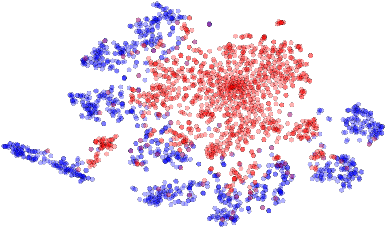
\includegraphics[width=0.45\textwidth]{Chapters/gradrev/figures/adaptation_vis/pool2_mnist2inv_before.pdf}}\hfill%
  \subfloat[Adapted]{%%
    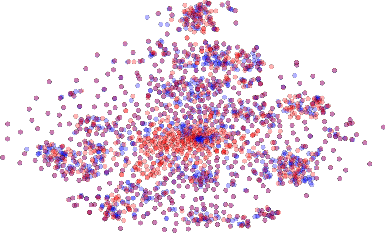
\includegraphics[width=0.45\textwidth]{Chapters/gradrev/figures/adaptation_vis/pool2_mnist2inv_after.pdf}}%%
%  \hspace*{\fill}%
%  \end{minipage}
%  \begin{minipage}{.45\textwidth}
%  \centering

\medskip
%   \small{{\sc Syn Numbers $ \rightarrow $ SVHN}: last hidden layer of the label predictor}\\
%   \setcounter{subfigure}{0}
% %  \hspace*{\fill}%
%   \subfloat[Non-adapted]{%%
%     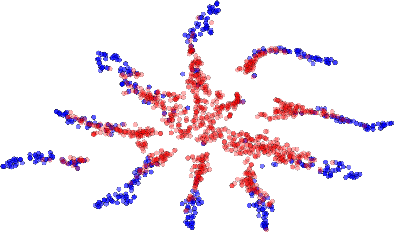
\includegraphics[width=0.45\textwidth]{Chapters/gradrev/figures/adaptation_vis/before.pdf}}\hfill%
%   \subfloat[Adapted]{%%
%     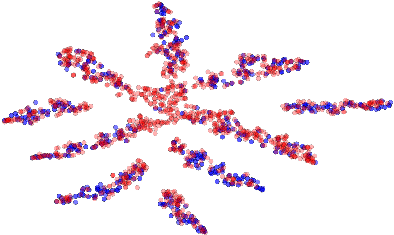
\includegraphics[width=0.45\textwidth]{Chapters/gradrev/figures/adaptation_vis/after.pdf}}%%
% %  \hspace*{\fill}%
% %  \end{minipage}
  \caption{The effect of adaptation on the distribution of the extracted features (best viewed in color). The figure shows t-SNE \citep{maaten2008visualizing} visualizations of the CNN's activations {\bf (a)} in case when no adaptation was performed and {\bf (b)} in case when our adaptation procedure was incorporated into training. {\it Blue} points correspond to the source domain examples, while {\it red} ones correspond to the target domain. In all cases, the adaptation in our method makes the two distributions of features much closer.}
  \label{fig:exper_adapt_vis}
\end{figure*}

\bigskip
\indent\textbf{Results}\\
%\subsubsection{Results On Image Data Sets}
\label{sect:exper_quant}
We now discuss the experimental settings and the results. In each case, we train on the source dataset and test on a different target domain dataset, with considerable shifts between domains (see \fig{exper_domains_examples}). The results are summarized in \tab{results}.% and \tab{results_office}. 

\vspace{2mm}\noindent {\bf MNIST $ \rightarrow $ MNIST-M}\\
%\subsubsection{MNIST $ \rightarrow $ MNIST-M}
Our first experiment deals with the MNIST dataset~\citep{LeCun98} (source). In order to obtain the target domain ({\sc MNIST-M}) we blend digits from the original set over patches randomly extracted from color photos from BSDS500 \citep{Arbelaez11}. This operation is formally defined for two images $ I^{1}, I^{2} $ as $ I_{ijk}^{out} = | I_{ijk}^{1} - I_{ijk}^{2} | $, where $ i, j $ are the coordinates of a pixel and $ k $ is a channel index. In other words, an output sample is produced by taking a patch from a photo and inverting its pixels at positions corresponding to the pixels of a digit. For a human the classification task becomes only slightly harder compared to the original dataset (the digits are still clearly distinguishable) whereas for a CNN trained on MNIST this domain is quite distinct, as the background and the strokes are no longer constant. Consequently, the source-only model performs poorly. Our approach succeeded at aligning feature distributions (\fig{exper_adapt_vis}), which led to successful adaptation results (considering that the adaptation is unsupervised). At the same time, the improvement over source-only model achieved by subspace alignment (SA) \citep{Fernando13} is quite modest, thus highlighting the difficulty of the adaptation task. 

% \vspace{2mm}\noindent {\bf Synthetic numbers $ \rightarrow $ SVHN.}
% %\subsubsection{Synthetic Numbers $ \rightarrow $ SVHN}
% To address a common scenario of training on synthetic data and testing on  real data, we use Street-View House Number dataset {\sc SVHN} \citep{Netzer11} as the target domain and synthetic digits as the source. The latter ({\sc Syn ~Numbers}) consists of $\approx \num[group-separator={,}]{500000}$ images generated by ourselves from Windows\textsuperscript{\tiny TM} fonts by varying the text (that includes different one-, two-, and three-digit numbers), positioning, orientation, background and stroke colors, and the amount of blur. The degrees of variation were chosen manually to simulate {\sc SVHN}, however the two datasets are still rather distinct, the biggest difference being the structured clutter in the background of {\sc SVHN} images. 

% The proposed backpropagation-based technique works well covering almost 80\% of the gap between training with source data only and training on target domain data with known target labels. In contrast, SA~\citep{Fernando13} results in a slight classification accuracy drop (probably due to the information loss during the dimensionality reduction), indicating that the adaptation task is even more challenging than in the case of the {\sc MNIST} experiment.

% \vspace{2mm}\noindent {\bf MNIST $ \leftrightarrow $ SVHN.}
% %\subsubsection{MNIST $ \leftrightarrow $ SVHN}
% In this experiment, we further increase the gap between distributions, and test on {\sc MNIST} and {\sc SVHN}, which are significantly different in appearance. Training on SVHN even without adaptation is challenging --- classification error stays high during the first 150 epochs. In order to avoid ending up in a poor local minimum we, therefore, do not use learning rate annealing here. Obviously, the two directions ({\sc MNIST} $ \rightarrow $ {\sc SVHN} and {\sc SVHN} $ \rightarrow $ {\sc MNIST}) are not equally difficult. As {\sc SVHN} is more diverse, a model trained on SVHN is expected to be more generic and to perform reasonably on the MNIST dataset. This, indeed, turns out to be the case and is supported by the appearance of the feature distributions. We observe a quite strong separation between the domains when we feed them into the CNN trained solely on {\sc MNIST}, whereas for the {\sc SVHN}-trained network the features are much more intermixed. This difference probably explains why our method succeeded in improving the performance by adaptation in the {\sc SVHN} $ \rightarrow $ {\sc MNIST} scenario (see \tab{results}) but not in the opposite direction (SA is not able to perform adaptation in this case either). Unsupervised adaptation from {\sc MNIST} to {\sc SVHN} gives a failure example for our approach: it doesn't manage to improve upon the performance of the non-adapted model which achieves $\approx 0.25$ accuracy (we are unaware of any unsupervised DA methods capable of performing such adaptation).

% \vspace{2mm}\noindent {\bf Synthetic Signs $ \rightarrow $ GTSRB.}
% %\subsubsection{Synthetic Signs $ \rightarrow $ GTSRB}
% Overall, this setting is similar to the {\sc Syn Numbers} $ \rightarrow $ {\sc SVHN} experiment, except the distribution of the features is more complex due to the significantly larger number of classes (43 instead of 10). For the source domain we obtained $ \num[group-separator={,}]{100000} $ synthetic images (which we call {\sc Syn~Signs}) simulating various imaging conditions. In the target domain, we use $ \num[group-separator={,}]{31367} $ random training samples for unsupervised adaptation and the rest for evaluation. Once again, our method achieves a sensible increase in performance proving its suitability for the synthetic-to-real data adaptation.

% \begin{figure}
%   \centering
%   \setlength\figureheight{4cm}
%   \setlength\figurewidth{6.8cm}
%   \input{Chapters/gradrev/figures/gtsrb_semi_2.tikz}
%   \caption{Results for the traffic signs classification in the semi-supervised setting. {\it Syn} and {\it Real} denote available labeled data ($ \num[group-separator={,}]{100000} $ synthetic and $430$ real images respectively); {\it Adapted} means that $\approx \num[group-separator={,}]{31000}$ unlabeled target domain images were used for adaptation. The best performance is achieved by employing both the labeled samples and the large unlabeled corpus in the target domain.}
%   \label{fig:exper_semi_test}
% \end{figure}

% As an additional experiment, we also evaluate the proposed algorithm for semi-supervised domain adaptation, \ie, when one is additionally provided with a small amount of labeled target data. Here, we reveal $430$ labeled examples (10 samples per class) and add them to the training set for the label predictor. \fig{exper_semi_test} shows the change of the validation error throughout the training. While the graph clearly suggests that our method can be beneficial in the semi-supervised setting, thorough verification of semi-supervised setting is left for future work.


%\vspace{2mm}\noindent {\bf Office dataset.} 
%\subsubsection{Office Data Set}
% We finally evaluate our method on {\sc Office} dataset, which is a collection of three distinct domains: {\sc Amazon}, {\sc DSLR}, and {\sc Webcam}. Unlike previously discussed datasets, {\sc Office} is rather small-scale with only 2817 labeled images spread across 31 different categories in the largest domain. The amount of available data is crucial for a successful training of a deep model, hence we opted for the fine-tuning of the CNN pre-trained on the ImageNet \citep{Jia14} as it is done in some recent DA works \citep{Donahue14,Tzeng14,Hoffman14}. We make our approach more comparable with \citet{Tzeng14} by using exactly the same network architecture replacing domain mean-based regularization with the domain classifier.
%
% Following most previous works, we evaluate our method using 5 random splits for each of the 3 transfer tasks commonly used for evaluation. Our training protocol is close to \citet{Tzeng14,Saenko10,Gong12} as we use the same number of labeled source-domain images per category. Unlike those works and similarly to DLID~\citep{Chopra13}, we use the whole unlabeled target domain (as the premise of our method is the abundance of unlabeled data in the target domain). Under this transductive setting, our method is able to improve previously-reported state-of-the-art accuracy for unsupervised adaptation very considerably (\tab{results_office}), especially in the most challenging {\sc Amazon} $ \rightarrow $ {\sc Webcam} scenario (the two domains with the largest domain shift).
%
% We finally evaluate our method on {\sc Office} dataset, which is a collection of three distinct domains: {\sc Amazon}, {\sc DSLR}, and {\sc Webcam}. Unlike previously discussed datasets, {\sc Office} is rather small-scale with only 2817 labeled images spread across 31 different categories in the largest domain. The amount of available data is crucial for a successful training of a deep model, hence we opted for the fine-tuning of the CNN pre-trained on the ImageNet (\texttt{AlexNet} from the \texttt{Caffe} package \citep{Jia14}) as it is done in some recent DA works \citep{Donahue14,Tzeng14,Hoffman14,Long15}. We make our approach more comparable with \cite{Tzeng14} by using exactly the same network architecture replacing domain mean-based regularization with the domain classifier.

% Following previous works, we assess the performance of our method across three transfer tasks most commonly used for evaluation. Our training protocol is adopted from \citep{Gong13,Chopra13,Long15} as during adaptation we use all available labeled source examples and unlabeled target examples (the premise of our method is the abundance of unlabeled data in the target domain). Also, all source domain data are used for training. Under this ``fully-transductive'' setting, our method is able to improve previously-reported state-of-the-art accuracy for unsupervised adaptation very considerably (\tab{results_office}), especially in the most challenging {\sc Amazon} $ \rightarrow $ {\sc Webcam} scenario (the two domains with the largest domain shift). 

% Interestingly, in all three experiments we observe a slight over-fitting (performance on the target domain degrades while accuracy on the source continues to improve) as training progresses, however, it doesn't ruin the validation accuracy. Moreover, switching off the domain classifier branch makes this effect far more apparent, from which we conclude that our technique serves as a regularizer.

\bigskip\indent\textbf{Experiments with deep image descriptors for re-identification}

% In this section we discuss the application of the described adaptation method to person re-identification \textit{(re-id}) problem.  The task of person re-identification is to associate people seen from different camera views. More formally, it can be defined as follows: given two sets of images from different cameras (\textit{probe} and \textit{gallery}) such that each person depicted in the probe set has an image in the gallery set,  for each image of a person from the probe set find an image of the same person in the gallery set.  Disjoint camera views, different illumination conditions, various poses and low quality of data make this problem difficult  even for humans (\eg, \citet{LiuLGW13} reports human performance at Rank1=$71.08\%$).  

% Unlike classification problems that are discussed above, re-identification problem implies that each image is mapped to a vector descriptor. The distance between descriptors is then used to match images from the probe set and the gallery set.
% To evaluate results of re-id methods the \textit{Cumulative Match Characteristic} (CMC) curve is commonly used. It is a plot of the identification rate (recall) at rank-$k$, that is the probability of the matching gallery image to be within the closest $k$ images (in terms of descriptor distance) to the probe image.

% Most existing works train descriptor mappings and evaluate them within the same dataset containing images from a certain camera network with similar imaging conditions. Several papers, however, observed that the performance of the resulting re-identification systems drops very considerably when descriptors trained on one dataset and tested on another. It is therefore natural to handle such cross-domain evaluation as a domain-adaptation problem, where each camera network (dataset) constitutes a domain.

% Recently, several papers  with significantly improved re-identification performance \citep{ZhangS14a,ZhaoOW14,Paisitkriangkrai15} have been presented, with \citet{MaLYL15} reporting good results in cross-data-set evaluation scenario. At the moment, deep learning methods \citep{Yi14} do not achieve state-of-the-art results probably because of the limited size of the training sets. Domain adaptation thus represents a viable direction for improving deep re-identification descriptors.

\bigskip
\indent\textbf{Datasets}\\
%\subsubsection{Datasets} 
%Following \citet{MaLYL15}, 
For cross-domain experiments, we use PRID \citep{Hirzer_h.:person}, VIPeR \citep{Gray07evaluatingappearance}, CUHK02 \citep{li2013locally} as target datasets for our experiments.  The \textit{PRID} dataset exists in two versions, we use a single-shot variant. 
We use all images in the first  pair of cameras of CUHK02 instead of choosing one image of a person from each camera view.  We refer to the subset of this dataset that includes the first pair of cameras only as \textit{CUHK02/p1} (as most papers use this subset). We also performed two experiments with all images of the whole CUHK02 dataset as source domain and VIPeR and PRID datasets as target domains similar to \citep{Yi14}.

%The \textit{PRID} dataset contains images of $385$ persons viewed from camera A and images of $749$ persons viewed from camera B,  $200$ persons appear in both cameras. The \textit{VIPeR} dataset also contains images taken with two cameras, and in total $632$ persons are captured, for every person there is one image for each of the two camera views. The \textit{CUHK02} dataset consists of images from five pairs of cameras, two images for each person from each of the two cameras. We refer to the subset of this dataset that includes the first pair of cameras only as \textit{CUHK02/p1} (as most papers use this subset).

 We perform extensive experiments for various pairs of datasets, where one dataset serves as a source domain, \ie, it is used to train a descriptor mapping in a supervised way with known correspondences between probe and gallery images. The second dataset is used as a target domain, so that images from that dataset are used without probe-gallery correspondence.

 In more detail, CUHK02/p1 is used for experiments when CUHK02 serves as a target domain and two settings (``whole CUHK02'' and CUHK02/p1) are used for experiments when CUHK02 serves as a source domain. Given PRID as a target dataset, we randomly choose $100$ persons appearing in both camera views as training set. The images of the other $100$ persons from camera A are used as probe, all images from camera B excluding those used in training ($649$ in total) are used as gallery at test time. For VIPeR, we use random 316 persons for training and all others for testing. For CUHK02, $971$ persons are split into $485$ for training and $486$ for testing.
 
We use all images in the first  pair of cameras of CUHK02 instead of choosing one image of a person from each camera view. We also performed two experiments with all images of the whole CUHK02 dataset as source domain and VIPeR and PRID datasets as target domains as in the  original paper \citep{Yi14}.
\newlength\reidheight
\setlength{\reidheight}{2.5cm}

\addtolength{\tabcolsep}{-3pt}

% \begin{figure*}
% \centering
% \begin{tabular}{cccc|cccc|cccc}
% 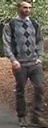
\includegraphics[height=\reidheight]{Chapters/gradrev/figures/dataset_samples/viper/a/000_45.png}&
% 
\includegraphics[height=\reidheight]{Chapters/gradrev/figures/dataset_samples/viper/b/000_45.png}&
% 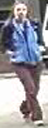
\includegraphics[height=\reidheight]{Chapters/gradrev/figures/dataset_samples/viper/a/001_45.png}&
% 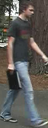
\includegraphics[height=\reidheight]{Chapters/gradrev/figures/dataset_samples/viper/b/002_90.png}&
% 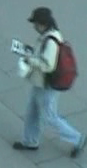
\includegraphics[height=\reidheight]{Chapters/gradrev/figures/dataset_samples/PRID/a/img_0001.png}&
% 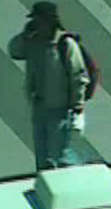
\includegraphics[height=\reidheight]{Chapters/gradrev/figures/dataset_samples/PRID/b/img_0001.png}&
% 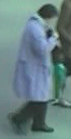
\includegraphics[height=\reidheight]{Chapters/gradrev/figures/dataset_samples/PRID/a/img_0002.png}&
% 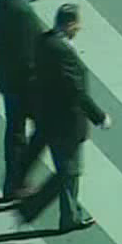
\includegraphics[height=\reidheight]{Chapters/gradrev/figures/dataset_samples/PRID/b/img_0003.png}&
% \includegraphics[height=\reidheight]{Chapters/gradrev/figures/dataset_samples/CUHK02/a/001_00005.png}&
% \includegraphics[height=\reidheight]{Chapters/gradrev/figures/dataset_samples/CUHK02/b/001_00221.png}&
% \includegraphics[height=\reidheight]{Chapters/gradrev/figures/dataset_samples/CUHK02/a/002_00280.png}&
% \includegraphics[height=\reidheight]{Chapters/gradrev/figures/dataset_samples/CUHK02/b/003_00403.png}\\
% \multicolumn{4}{c}{VIPER}&
% \multicolumn{4}{c}{PRID}&
% \multicolumn{4}{c}{CUHK02}
% \end{tabular}
% \caption{Matching and non-matching pairs of probe-gallery images from different person re-identification datasets. The three datasets are treated as different domains in our experiments.}
% \label{fig:reidsamples}
% \end{figure*}

\addtolength{\tabcolsep}{3pt}

Following \citet{Yi14}, we augmented our data with mirror images, and during test time we calculate similarity score between two images as the mean of the four scores corresponding to different flips of the two compared images. In case of CUHK02, where there are four images (including mirror images) for each of the two camera views for each person, all $16$ combinations' scores are averaged. 

\bigskip
\indent\textbf{CNN architectures and Training Procedure}\\
%\subsubsection{CNN architectures and Training Procedure} 
In our experiments, we use DML siamese architecture \citep{Yi14} described in \sect{intro_architectures}. %(\textit{Deep Metric Learning} or \textit{DML}) for learning deep image descriptors on the source dataset.
% This architecture incorporates two convolution layers (with $7\times7$ and $5\times5$ filter banks), followed by ReLU and max pooling, and one fully-connected layer, which gives $500$-dimensional descriptors as an output. There are three parallel flows within the CNN for processing three part of an image: the upper, the middle, and the lower one. The first convolution layer shares parameters between three parts, and the outputs of the second convolution layers are concatenated.
% During training, we follow \citet{Yi14} and calculate pairwise cosine similarities between $500$-dimensional features within each batch and backpropagate the loss for all pairs within batch. 

To perform domain-adversarial training, we construct a DANN architecture.  The feature extractor includes the two convolutional layers (followed by max-pooling and ReLU) discussed above. The label predictor in this case is replaced with \textit{descriptor predictor} that includes one fully-connected layer. The domain classifier includes two fully-connected layers with $500$ units in the intermediate representation ($x{\rightarrow}500{\rightarrow}1$). 

For the verification loss function in the descriptor predictor we used Binomial Deviance loss \eq{bindev}, also used in \citet{Yi14} with similar parameters: $\alpha = 2$, $\beta = 0.5$, $c = 2$ (the asymmetric cost parameter for negative pairs). The domain classifier is trained with logistic loss as in \sect{experiments}.

We used learning rate fixed to $0.001$ and momentum of $0.9$. The schedule of adaptation similar to the one described in \sect{experiments} was used. We also inserted dropout layer with rate $0.5$ after the concatenation of outputs of the second max-pooling layer. $128$-sized batches were used for source data and $128$-sized batches for target data. 

%TODO fix 
% \begin{figure*}[t]
%   \definecolor{fnodebottom}{RGB}{132,170,81}
%   \definecolor{fnodetop}{RGB}{172,222,106}
%   \definecolor{cnodebottom}{RGB}{120,128,164}
%   \definecolor{cnodetop}{RGB}{158,167,218}
%   \definecolor{dnodebottom}{RGB}{174,109,146}
%   \definecolor{dnodetop}{RGB}{230,141,192}
%   \centering
%   {%
%      \scalebox{0.65}{\input{Chapters/gradrev/archs/reidentification_adaptation.tikz}}}\\
%   \caption{CNN architecture used in experiments on domain adaptation for person re-identification}
%   \label{fig:reid_arch}
% \end{figure*}

\bigskip
\indent\textbf{Results}
%\subsubsection{Results on Re-identification datasets} 
\begin{figure}[t]
\centering
  \begin{tabular}{p{5cm}  p{5cm}  p{5cm} }
      
        \setlength\figureheight{3.5cm}
        \setlength\figurewidth{3.5cm}
        \begin{tikzpicture}[font=\scriptsize]

\begin{axis}[%
width=0.95092\figurewidth,
height=\figureheight,
at={(0\figurewidth,0\figureheight)},
scale only axis,
xmin=1,
xmax=50,
xlabel={Rank},
ymin=0,
ymax=1,
ylabel={Identification rate (\%)},
axis x line*=bottom,
axis y line*=left,
legend style={at={($ (0,1) + (+0.1cm,+0.1cm) $)},anchor=north west,align=left,legend cell align=left,draw=black},
xmajorgrids,
ymajorgrids,
grid style={dashed}
]
\addplot [color=blue,solid,line width=1.0pt]
  table[row sep=crcr]{%
1    0.1518987341772152\\
5    0.34810126582278483\\
10   0.47468354430379744\\
15   0.5474683544303798\\
20   0.5886075949367089\\
25   0.629746835443038\\
30   0.6613924050632911\\
35   0.680379746835443\\
40   0.7120253164556962\\
45   0.7183544303797469\\
50   0.7310126582278481\\
};
\addlegendentry{DML};

\addplot [color=cyan,solid,line width=1.0pt]
  table[row sep=crcr]{%
1    0.14556962025316456\\
5    0.3322784810126582\\
10   0.4873417721518987\\
15   0.5569620253164557\\
20   0.5917721518987342\\
25   0.6424050632911392\\
30   0.689873417721519\\
35   0.7025316455696202\\
40   0.7278481012658228\\
45   0.7531645569620253\\
50   0.7848101265822784\\
};
\addlegendentry{DML, adaptation};



\end{axis}
\end{tikzpicture}%
        \centering\small{(a) Whole CUHK02 $\rightarrow$ VIPeR}
        \label{fig:allcuhk_viper}
  
    &
        \setlength\figureheight{3.5cm}
        \setlength\figurewidth{3.5cm}
        \begin{tikzpicture}[font=\scriptsize]

\begin{axis}[%
width=0.95092\figurewidth,
height=\figureheight,
at={(0\figurewidth,0\figureheight)},
scale only axis,
xmin=1,
xmax=50,
xlabel={Rank},
ymin=0,
ymax=1,
ylabel={Identification rate (\%)},
axis x line*=bottom,
axis y line*=left,
legend style={at={($ (0,1) + (+0.1cm,+0.1cm) $)},anchor=north west,align=left,legend cell align=left,draw=black},
xmajorgrids,
ymajorgrids,
grid style={dashed}
]
\addplot [color=blue,solid,line width=1.0pt]
  table[row sep=crcr]{%
1      0.126582278481 \\
5      0.303797468354 \\
10      0.414556962025 \\
15      0.490506329114 \\
20      0.550632911392 \\
25      0.613924050633 \\
30      0.651898734177 \\
35      0.686708860759 \\
40      0.708860759494 \\
45      0.75 \\
50      0.759493670886 \\
};
\addlegendentry{DML};

\addplot [color=cyan,solid,line width=1.0pt]
  table[row sep=crcr]{%
1      0.120253164557 \\
5      0.29746835443 \\
10      0.462025316456 \\
15      0.541139240506 \\
20      0.594936708861 \\
25      0.617088607595 \\
30      0.645569620253 \\
35      0.667721518987 \\
40      0.696202531646 \\
45      0.712025316456 \\
50      0.73417721519 \\
};
\addlegendentry{DML, adaptation};


\end{axis}
\end{tikzpicture}%
        \centering\small{(b) CUHK02/p1 $\rightarrow$ VIPeR}
%        \label{fig:CUHK02_p1_viper}
    &
        \setlength\figureheight{3.5cm}
        \setlength\figurewidth{3.5cm}
        \begin{tikzpicture}[font=\scriptsize]

\begin{axis}[%
width=0.95092\figurewidth,
height=\figureheight,
at={(0\figurewidth,0\figureheight)},
scale only axis,
xmin=1,
xmax=50,
xlabel={Rank},
ymin=0,
ymax=1,
ylabel={Identification rate (\%)},
axis x line*=bottom,
axis y line*=left,
legend style={at={($ (0,1) + (+0.1cm,+0.1cm) $)},anchor=north west,align=left,legend cell align=left,draw=black},
xmajorgrids,
ymajorgrids,
grid style={dashed}
]
\addplot [color=blue,solid,line width=1.0pt]
  table[row sep=crcr]{%
1      0.0664556962025 \\
5      0.167721518987 \\
10      0.253164556962 \\
15      0.275316455696 \\
20      0.316455696203 \\
25      0.348101265823 \\
30      0.379746835443 \\
35      0.414556962025 \\
40      0.45253164557 \\
45      0.474683544304 \\
50      0.496835443038 \\
};
\addlegendentry{DML};

\addplot [color=cyan,solid,line width=1.0pt]
  table[row sep=crcr]{%
1      0.0632911392405 \\
5      0.161392405063 \\
10      0.259493670886 \\
15      0.338607594937 \\
20      0.389240506329 \\
25      0.417721518987 \\
30      0.439873417722 \\
35      0.471518987342 \\
40      0.496835443038 \\
45      0.518987341772 \\
50      0.53164556962 \\
};
\addlegendentry{DML, adaptation};


\end{axis}
\end{tikzpicture}%
        \centering\small{(c) PRID $\rightarrow$ VIPeR}
%        \label{fig:CUHK02_p1_viper} \\    
 \end{tabular}
%  \caption{Results on VIPeR}
%  \label{fig:viper}
% \end{figure}%

% \begin{figure}[h]
% \centering
 \begin{tabular}{ p{5cm}  p{5cm}  p{5cm} }
        \setlength\figureheight{3.5cm}
        \setlength\figurewidth{4cm}
        \begin{tikzpicture}[font=\scriptsize]

\begin{axis}[%
width=0.95092\figurewidth,
height=\figureheight,
at={(0\figurewidth,0\figureheight)},
scale only axis,
xmin=1,
xmax=50,
xlabel={Rank},
ymin=0,
ymax=1,
ylabel={Identification rate (\%)},
axis x line*=bottom,
axis y line*=left,
legend style={at={($ (0,1) + (+0.1cm,+0.1cm) $)},anchor=north west,align=left,legend cell align=left,draw=black},
xmajorgrids,
ymajorgrids,
grid style={dashed}
]
\addplot [color=blue,solid,line width=1.0pt]
  table[row sep=crcr]{%
1    0.08\\
5    0.13\\
10   0.22\\
15   0.27\\
20   0.31\\
25   0.35\\
30   0.4\\
35   0.41\\
40   0.41\\
45   0.43\\
50   0.44\\
};
\addlegendentry{DML};

\addplot [color=cyan,solid,line width=1.0pt]
  table[row sep=crcr]{%
1    0.07\\
5    0.19\\
10   0.27\\
15   0.32\\
20   0.35\\
25   0.37\\
30   0.39\\
35   0.41\\
40   0.43\\
45   0.45\\
50   0.45\\
};
\addlegendentry{DML, adaptation};


%[0.08, 0.13, 0.22, 0.27, 0.31, 0.35, 0.4, 0.41, 0.41, 0.43, 0.44]
%[0.07, 0.19, 0.27, 0.32, 0.35, 0.37, 0.39, 0.41, 0.43, 0.45, 0.45]

%
\end{axis}
\end{tikzpicture}%





        \centering\small{(d) Whole CUHK02 $\rightarrow$ PRID}
        \label{fig:allcuhk_prid}
    &
        \setlength\figureheight{3.5cm}
        \setlength\figurewidth{4cm}
        \begin{tikzpicture}[font=\scriptsize]

\begin{axis}[%
width=0.95092\figurewidth,
height=\figureheight,
at={(0\figurewidth,0\figureheight)},
scale only axis,
xmin=1,
xmax=50,
xlabel={Rank},
ymin=0,
ymax=1,
ylabel={Identification rate (\%)},
axis x line*=bottom,
axis y line*=left,
legend style={at={($ (0,1) + (+0.1cm,+0.1cm) $)},anchor=north west,align=left,legend cell align=left,draw=black},
xmajorgrids,
ymajorgrids,
grid style={dashed}
]
\addplot [color=blue,solid,line width=1.0pt]
  table[row sep=crcr]{%
1      0.04 \\
5      0.08 \\
10      0.15 \\
15      0.22 \\
20      0.25 \\
25      0.3 \\
30      0.32 \\
35      0.36 \\
40      0.39 \\
45      0.41 \\
50      0.44 \\
};
\addlegendentry{DML};

\addplot [color=cyan,solid,line width=1.0pt]
  table[row sep=crcr]{%
1      0.06 \\
5      0.16 \\
10      0.21 \\
15      0.27 \\
20      0.31 \\
25      0.36 \\
30      0.39 \\
35      0.41 \\
40      0.41 \\
45      0.42 \\
50      0.43 \\
};
\addlegendentry{DML, adaptation};


\end{axis}
\end{tikzpicture}%
        \centering\small{(e) CUHK02/p1 $\rightarrow$ PRID}
        \label{fig:CUHK02_p1_prid}
    &
       \setlength\figureheight{3.5cm}
       \setlength\figurewidth{4cm}
       \begin{tikzpicture}[font=\scriptsize]

\begin{axis}[%
width=0.95092\figurewidth,
height=\figureheight,
at={(0\figurewidth,0\figureheight)},
scale only axis,
xmin=1,
xmax=50,
xlabel={Rank},
ymin=0,
ymax=1,
ylabel={Identification rate (\%)},
axis x line*=bottom,
axis y line*=left,
legend style={at={($ (0,1) + (+0.1cm,+0.1cm) $)},anchor=north west,align=left,legend cell align=left,draw=black},
xmajorgrids,
ymajorgrids,
grid style={dashed}
]
\addplot [color=blue,solid,line width=1.0pt]
  table[row sep=crcr]{%
1      0.08 \\
5      0.15 \\
10      0.19 \\
15      0.25 \\
20      0.28 \\
25      0.34 \\
30      0.35 \\
35      0.36 \\
40      0.39 \\
45      0.4 \\
50      0.41 \\
};
\addlegendentry{DML};

\addplot [color=cyan,solid,line width=1.0pt]
  table[row sep=crcr]{%
1      0.07 \\
5      0.19 \\
10      0.25 \\
15      0.27 \\
20      0.31 \\
25      0.36 \\
30      0.39 \\
35      0.42 \\
40      0.42 \\
45      0.46 \\
50      0.47 \\
};
\addlegendentry{DML, adaptation};


\end{axis}
\end{tikzpicture}%
        \centering\small{(f) VIPeR $\rightarrow$ PRID}
        \label{fig:viper_prid}  \\    
 \end{tabular}
%  \caption{Results on PRID}
%  \label{fig:prid}
% \end{figure}


% \begin{figure}[h]
% \centering
 \begin{tabular}{ p{5cm}  p{5cm}}
        \setlength\figureheight{3.5cm}
        \setlength\figurewidth{4cm}
        \begin{tikzpicture}[font=\scriptsize]

\begin{axis}[%
width=0.95092\figurewidth,
height=\figureheight,
at={(0\figurewidth,0\figureheight)},
scale only axis,
xmin=1,
xmax=50,
xlabel={Rank},
ymin=0,
ymax=1,
ylabel={Identification rate (\%)},
axis x line*=bottom,
axis y line*=left,
legend style={at={($ (0,1) + (+0.1cm,+0.1cm) $)},anchor=north west,align=left,legend cell align=left,draw=black},
xmajorgrids,
ymajorgrids,
grid style={dashed}
]
\addplot [color=blue,solid,line width=1.0pt]
  table[row sep=crcr]{%
1      0.109053497942 \\
5      0.265432098765 \\
10      0.366255144033 \\
15      0.407407407407 \\
20      0.465020576132 \\
25      0.491769547325 \\
30      0.510288065844 \\
35      0.541152263374 \\
40      0.572016460905 \\
45      0.59670781893 \\
50      0.617283950617 \\
};
\addlegendentry{DML};

\addplot [color=cyan,solid,line width=1.0pt]
  table[row sep=crcr]{%
1      0.125514403292 \\
5      0.253086419753 \\
10      0.366255144033 \\
15      0.440329218107 \\
20      0.5 \\
25      0.5329218107 \\
30      0.572016460905 \\
35      0.594650205761 \\
40      0.617283950617 \\
45      0.650205761317 \\
50      0.668724279835 \\
};
\addlegendentry{DML, adaptation};


\end{axis}
\end{tikzpicture}%
        \centering\small{(g) VIPeR $\rightarrow$ CUHK02/p1}
        \label{fig:viper_CUHK02_p1}
    &
        \setlength\figureheight{3.5cm}
        \setlength\figurewidth{4cm}
        \begin{tikzpicture}[font=\scriptsize]

\begin{axis}[%
width=0.95092\figurewidth,
height=\figureheight,
at={(0\figurewidth,0\figureheight)},
scale only axis,
xmin=1,
xmax=50,
xlabel={Rank},
ymin=0,
ymax=1,
ylabel={Identification rate (\%)},
axis x line*=bottom,
axis y line*=left,
legend style={at={($ (0,1) + (+0.1cm,+0.1cm) $)},anchor=north west,align=left,legend cell align=left,draw=black},
xmajorgrids,
ymajorgrids,
grid style={dashed}
]
\addplot [color=blue,solid,line width=1.0pt]
  table[row sep=crcr]{%
1      0.0569620253165 \\
5      0.139240506329 \\
10      0.212025316456 \\
15      0.284810126582 \\
20      0.316455696203 \\
25      0.344936708861 \\
30      0.370253164557 \\
35      0.389240506329 \\
40      0.414556962025 \\
45      0.443037974684 \\
50      0.465189873418 \\
};
\addlegendentry{DML};

\addplot [color=cyan,solid,line width=1.0pt]
  table[row sep=crcr]{%
1      0.0843621399177 \\
5      0.191358024691 \\
10      0.263374485597 \\
15      0.316872427984 \\
20      0.347736625514 \\
25      0.395061728395 \\
30      0.432098765432 \\
35      0.471193415638 \\
40      0.504115226337 \\
45      0.5329218107 \\
50      0.553497942387 \\
};
\addlegendentry{DML, adaptation};


\end{axis}
\end{tikzpicture}%
        \centering\small{(h) PRID $\rightarrow$ CUHK02/p1}
        \label{fig:prid_CUHK02_p1}
  \\    
  \end{tabular}
  \caption{Results on VIPeR, PRID and CUHK02/p1 with and without domain-adversarial learning. Across the eight domain pairs domain-adversarial learning improves re-identification accuracy. For some domain pairs the improvement is considerable.}
  \label{fig:adaptresults}
\end{figure}

Figure \ref{fig:adaptresults} shows results in the form of Rekall@K metric for eight pairs of datasets. Depending on the hardness of the annotation problem we trained either for 50,000 iterations (CUHK02/p1 $\rightarrow$ VIPeR, VIPeR $\rightarrow$ CUHK02/p1, PRID $\rightarrow$ VIPeR) or for 20,000 iterations (the other five pairs). 

\begin{figure*}
\centering
\begin{tabular}{c c}
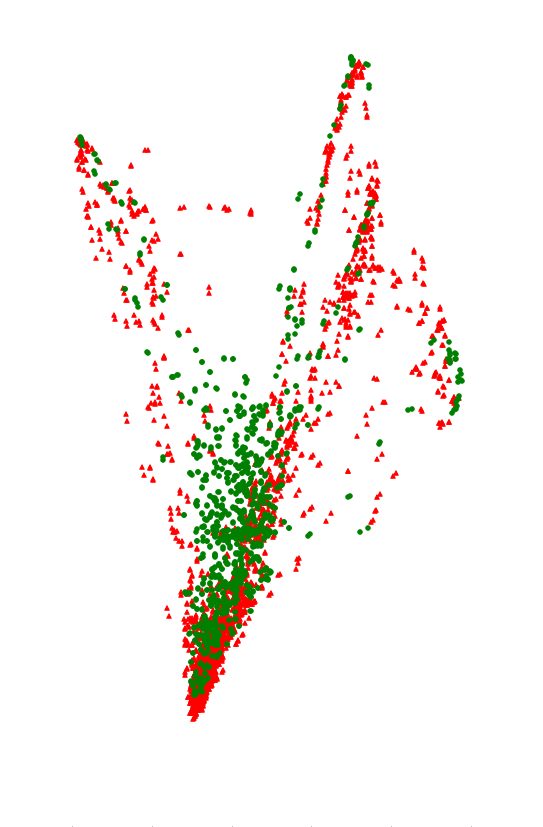
\includegraphics[height=7cm, width=7cm]{Chapters/gradrev/figures/reid_adapt_results/viper_cuhkp1_zc.png}&
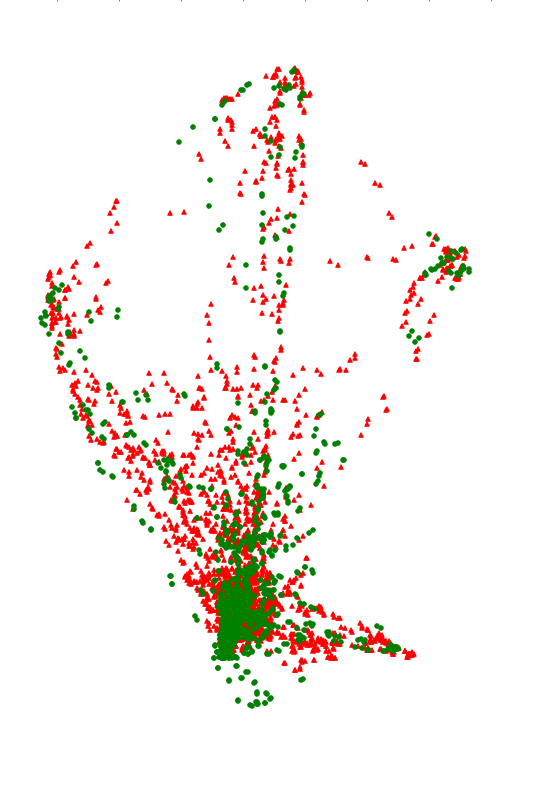
\includegraphics[height=7cm, width=7cm]{Chapters/gradrev/figures/reid_adapt_results/viper_cuhkp1_da.png}\\
\small{(a) DML}&
\small{(b) DML, adaptation}\\
\end{tabular}
\caption{The effect of adaptation shown by t-SNE visualizations of source and target domains descriptors in a VIPeR $\rightarrow$ CUHK02/p1 experiment pair. VIPeR is depicted with \textit{green} and CUHK02/p1 - with \textit{red}. As in the image classification case, domain-adversarial learning ensures a closer match between the source and the target distributions. }
\label{fig:reidtsne}
\end{figure*}


After the sufficient number of iterations, domain-adversarial training consistently improves the performance of re-identification. For the pairs that involve PRID dataset, which is more dissimilar to the other two datasets, the improvement is considerable. Overall, this demonstrates the applicability of the domain-adversarial learning beyond classification problems.

Figure \ref{fig:reidtsne} further demonstrates the effect of adaptation on the distributions of the learned descriptors in the source and in target sets in VIPeR $\rightarrow$ CUHK02/p1 experiments, where domain adversarial learning once again achieves better intermixing of the two domains.


\section{Conclusion}

The chapter describes a new approach to domain adaptation of feed-forward neural networks, which allows large-scale training based on large amount of annotated data in the source domain and large amount of unannotated data in the target domain. Similarly to many previous shallow and deep DA techniques, the adaptation is achieved through aligning the distributions of features across the two domains. However, unlike previous approaches, the alignment is accomplished through standard backpropagation training.

%The approach is motivated and supported by the domain adaptation theory of \citet{BenDavid-NIPS06}. 
 The main idea behind DANN is to enjoin the network hidden layer to learn a representation which is predictive of the source example labels, but uninformative about the domain of the input (source or target). 
% We implement this new approach within both shallow and deep feed-forward architectures. The latter allows simple implementation within virtually any deep learning package through the introduction of a simple gradient reversal layer. 
%We have shown that our approach is flexible and improves the results for classification tasks as well as person re-identification. 

A convenient aspect of our approach is that the domain adaptation component can be added to almost any neural network architecture that is trainable with backpropagation. Towards this end, we have demonstrated experimentally that the approach is not confined to classification tasks but can be used in other feed-forward architectures, e.g.\ for descriptor learning for person re-identification. The full set of experiments, including those for classification, is presented in the corresponding publication \citep{ganin2016domain}.

% Further evaluation on larger-scale tasks and in semi-supervised settings constitutes future work. It is also interesting whether the approach can benefit from a good initialization of the feature extractor. For this, a natural choice would be to use deep autoencoder/deconvolution network trained on both domains (or on the target domain) in the same vein as \citet{Glorot11,Chopra13}, effectively using \citet{Glorot11,Chopra13} as an initialization to our method.

%\pagebreak

% \acks{This work has been supported by National Science and Engineering Research Council (NSERC) Discovery
% grants 262067 and 0122405 as well as the Russian Ministry of Science and Education grant RFMEFI57914X0071.
% Computations were performed on the Colosse supercomputer grid at Universit\'e Laval, under the auspices of Calcul Qu\'ebec and Compute Canada. The operations of Colosse are funded by the NSERC, the Canada Foundation for Innovation (CFI), NanoQu\'ebec, and the Fonds de recherche du Qu\'ebec -- Nature et technologies (FRQNT). We also thank the Graphics \& Media Lab, Faculty of Computational Mathematics and Cybernetics, Lomonosov Moscow State University for providing the synthetic road signs dataset.}


% \iffalse

% \appendix

% \section{Shallow DANN Algorithm}
% \label{supmat:shallow_DANN}

% In the pseudocode of Algorithm~\ref{alg:stoch-up}, we use
% $\ee(y)$ to refer to a ``one-hot'' vector, consisting of all $0$s except for a $1$ at position~$y$. Also, $\odot$ is the element-wise product.
% %Notice that, on Line~\ref{algoline:da} of Algorithm~\ref{alg:stoch-up}, the....

% \iffalse
% To optimize Equation~\eqref{eqn:global}, one option would be to follow a hard-EM approach,
% where we would alternate between optimizing until convergence the adversarial parameters $\uu, d$ and the
% other regular neural network parameters $\WW, \VV, \bb, \cc$. However, we've found that a simpler stochastic gradient approach is sufficient and works well in practice. Here, the stochastic gradient approach consists in sampling a pair of source and target example $\xb_i, \xb_j$ and updating a gradient step update of all parameters of DANN. Crucially, while the update of the regular parameters follows as usual the opposite direction of the gradient, for the adversarial parameters $\uu, d$ the step must follow the gradient's direction (since we maximize with respect to them, instead of minimizing). 
% \fi 

% %\afterpage{
% \begin{algorithm}[t]
%   \caption{Shallow DANN -- Stochastic training update}
%   \label{alg:stoch-up}
% %   \algsetup{
% %   linenosize=\small,
% %   linenodelimiter=.
% %   }
% \begin{multicols}{2}
% \begin{algorithmic}[1]
% {\footnotesize
%   \STATE {\bfseries Input:} \\
%   --- samples $S=\{(\xb_i, \ys_i)\}_{i=1}^n$ and $T=\{\xb_i\}_{i=1}^{n'}$,\\
%   --- hidden layer size $D$, \\
%   --- adaptation parameter $\lambda$,\\
%   --- learning rate $\mu$,
%   \STATE {\bfseries Output:} neural network $\{\WW, \VV, \bb, \cc\}$ 
%   \vspace{2mm}
% %   \STATE 
%   \STATE $\WW, \VV \leftarrow {\rm random\_init}(\,D\,)$
%   \STATE $\bb, \cc, \uu, d \leftarrow 0$
%   \WHILE{stopping criteria is not met}
%   \FOR{$i$ from 1 to $n$}
%   \STATE \# {\tt Forward propagation}
%   \STATE $G_f(\xb_i) \leftarrow \sigm(\bb + \WW\xb_i)$
%   \STATE $G_y(G_f(\xb_i)) \leftarrow \softmax(\cc + \VV G_f(\xb_i))$
%   \vspace{1.5mm}
%   \STATE \# {\tt Backpropagation}
%   \STATE $\Delta_{\cc} \leftarrow -(\ee(\ys_i)-G_y(G_f(\xb_i)))$ 
%   % \# $\ee(y)$ is a ``one-hot'' vector, that is all 0s but with a 1 at position~$y$
%   \STATE $\Delta_{\VV} \leftarrow \Delta_{\cc}~G_f(\xb_i)^\top$ 
%   \STATE $\Delta_{\bb} \leftarrow \left(\VV^{\top} \Delta_{\cc}\right) \odot G_f(\xb_i) \odot (1-G_f(\xb_i))$
%   % \# $\odot$ is the element-wise product
%   \STATE $\Delta_{\WW} \leftarrow \Delta_{\bb} \cdot({\xb_i})^\top$
%   \vspace{1.5mm}
%   \STATE \# {\tt Domain adaptation regularizer...}
%   \STATE \# {\tt ...from current domain}
%   \STATE $G_d(G_f(\xb_i)) \leftarrow \sigm(d + \uu^\top G_f(\xb_i))$
%   \STATE $\Delta_d \leftarrow \lambda (1-G_d(G_f(\xb_i)))$ 
%   \STATE $\Delta_{\uu} \leftarrow \lambda(1-G_d(G_f(\xb_i))) G_f(\xb_i)$
%   \STATE ${\rm tmp} \leftarrow \lambda(1-G_d(G_f(\xb_i)))$\\*
%   ~~~~~~~~~~~~~~~${}\times\uu \odot G_f(\xb_i) \odot (1-G_f(\xb_i))$
%   \STATE $\Delta_{\bb} \leftarrow \Delta_{\bb} + {\rm tmp}$ 
%   \STATE $\Delta_{\WW} \leftarrow \Delta_{\WW} + {\rm tmp}\cdot({\xb_i})^\top$
%   \label{algoline:omit1}
%       \vspace{1.5mm}
%   \STATE \# {\tt ...from other domain}
%   \STATE $j \leftarrow {\rm uniform\_integer}(1,\dots,n')$
%   \STATE $G_f(\xb_j) \leftarrow \sigm(\bb + \WW\xb_j)$
%   \STATE $G_d(G_f(\xb_j)) \leftarrow \sigm(d + \uu^\top G_f(\xb_j))$ 
%   \STATE $\Delta_d \leftarrow \Delta_d - \lambda G_d(G_f(\xb_j))$
%   \STATE $\Delta_{\uu} \leftarrow \Delta_{\uu} - \lambda G_d(G_f(\xb_j)) G_f(\xb_j)$
%   \STATE ${\rm tmp} \leftarrow -\lambda G_d(G_f(\xb_j))$\\*
%   ~~~~~~~~~~~~~~~${}\times\uu \odot G_f(\xb_j) \odot (1-G_f(\xb_j))$
%   \STATE $\Delta_{\bb} \leftarrow \Delta_{\bb} + {\rm tmp}$ 
%   \STATE $\Delta_{\WW} \leftarrow \Delta_{\WW} + {\rm tmp}\cdot(\xb_j)^\top$
%   \label{algoline:omit2}
%       \vspace{1.5mm}
%   \STATE \# {\tt Update neural network parameters}
%   \STATE $\WW \leftarrow \WW - \mu \Delta_{\WW}$ 
%   \STATE $\VV \leftarrow \VV - \mu \Delta_{\VV}$
%   \STATE $\bb \leftarrow \bb - \mu \Delta_{\bb}$ 
%   \STATE $\cc \leftarrow \cc - \mu \Delta_{\cc}$
%       \vspace{1.5mm}
%   \STATE \# {\tt Update domain classifier}
% %   \STATE $\uu \leftarrow \uu + \mu \Delta_{\uu}$ \# Notice the ``+'' instead of the ``-''
% %   \STATE $d \leftarrow d + \mu \Delta_{d}$
%   \STATE $\uu \leftarrow \uu + \mu \Delta_{\uu}$ 
%   \STATE $d \leftarrow d + \mu \Delta_{d}$
%   \label{algoline:da}
%       \ENDFOR
%   \ENDWHILE
% %   \STATE 
% %   \RETURN $\{\WW, \VV, \bb, \cc\}$
%   } 
% \end{algorithmic}
% \end{multicols}
% \end{algorithm}
% %}

% \medskip


% \iffalse
% \section{An alternative optimization approach}
% \label{supmat:alternative_optimization}


% \def\x{{\mathbf x}}
% \def\f{{\mathbf f}}

% \def\S{{\cal S}}
% \def\T{{\cal T}}

% \def\R{{\mathds R}}

% \def\tf{{\theta_f}}
% \def\td{{\theta_d}}
% \def\ty{{\theta_y}}
% \def\htf{{\hat\theta_f}}
% \def\htd{{\hat\theta_d}}
% \def\hty{{\hat\theta_y}}

% There exists an alternative construction \citep[inspired by][]{Goodfellow14} that leads to the same updates \eq{upd1}-\eq{upd3}. Rather than using the gradient reversal layer, the construction introduces two different loss functions for the domain classifier. Minimization of the first domain loss ($ L_{d+} $) should lead to a better domain discrimination, while the second domain loss ($ L_{d-} $) is minimized when the domains are distinct. Stochastic updates for $ \theta_f $ and $ \theta_d $ are then defined as:
% \begin{align*}
%   \tf \quad &\longleftarrow \quad \tf \;-\; \mu \left(\frac{\partial \Lcal_y^i}{\partial \tf} + \frac{\partial \Lcal^i_{d-}}{\partial \tf} \right)\\
%   \td \quad &\longleftarrow \qquad \td \;-\; \mu \frac{\partial \Lcal^i_{d+}}{\partial \td} \, ,
% \end{align*}
% Thus, different parameters participate in the optimization of different losses

% In this framework, the gradient reversal layer constitutes a special case, corresponding  to the pair of domain losses $ (\Lcal_d, -\lambda \,\Lcal_d) $. However, other pairs of loss functions can be used. One example would be the binomial cross-entropy \citep{Goodfellow14}:
% \begin{equation*}
%   \Lcal_{d+}(q, d) = \sum_{i = 1..N} d_i \log(q_i) + (1 - d_i) \log(1 - q_i) \, ,
% \end{equation*}
% where $ d $ indicates domain indices and $ q $ is an output of the predictor. In that case ``adversarial'' loss is easily obtained by swapping domain labels, \ie, $ L_{d-}(q, d) = L_{d+}(q, 1 - d) $. This particular pair has a potential advantage of producing stronger gradients at early learning stages if the domains are quite dissimilar. In our experiments, however, we did not observe any significant improvement resulting from this choice of losses.
% \fi

% \iffalse
% \section{CNN architectures}
% \label{supmat:CNN}

% \begin{figure*}[t]
%   \definecolor{fnodebottom}{RGB}{132,170,81}
%   \definecolor{fnodetop}{RGB}{172,222,106}
%   \definecolor{cnodebottom}{RGB}{120,128,164}
%   \definecolor{cnodetop}{RGB}{158,167,218}
%   \definecolor{dnodebottom}{RGB}{174,109,146}
%   \definecolor{dnodetop}{RGB}{230,141,192}
%   \centering
%   \subfloat[MNIST architecture]{%
%     \scalebox{0.65}{\begin{tikzpicture}[
  black!50, text=black,
  node distance=4mm,
  grlnode/.style={
    align=center,
    circle,minimum size=6mm,
    inner sep=5pt,
    very thick,draw=black!50,
    font=\ttfamily
  },
  fnode/.style={
    align=center,
    % The shape:
    rectangle,minimum size=6mm,rounded corners,
    % The rest
    inner sep=5pt,
    very thick,draw=black!50,
    top color=fnodetop,bottom color=fnodebottom,
    font=\ttfamily},
  cnode/.style={
    fnode,top color=cnodetop,bottom color=cnodebottom},
  dnode/.style={
    fnode,top color=dnodetop,bottom color=dnodebottom},
  vhedge/.style={
    rounded corners,to path=|- (\tikztotarget)}]
  \matrix[row sep=5mm,column sep=5mm] {
    \node (conv1) [fnode] {conv 5x5\\32 maps\\ReLU}; &
    \node (pool1) [fnode] {max-pool 2x2\\2x2 stride}; &
    \node (conv2) [fnode] {conv 5x5\\48 maps\\ReLU}; &
    \node (pool2) [fnode] {max-pool 2x2\\2x2 stride}; &
  
    \node (fc3)   [cnode] {fully-conn\\100 units\\ReLU}; &
    \node (fc4)   [cnode] {fully-conn\\100 units\\ReLU}; &
    \node (fc5)   [cnode] {fully-conn\\10 units\\Soft-max}; \\
  
    & & &
    \node (grl) [grlnode] {GRL}; &
  
    \node (fc1_d) [dnode] {fully-conn\\100 units\\ReLU}; &
    \node (fc2_d) [dnode] {fully-conn\\1 unit\\Logistic}; \\
  };
  
  \path (conv1) edge[-latex,shorten >=1pt,very thick] (pool1);
  \path (pool1) edge[-latex,shorten >=1pt,very thick] (conv2);
  \path (conv2) edge[-latex,shorten >=1pt,very thick] (pool2);
  \path (pool2) edge[-latex,shorten >=1pt,very thick] (fc3);
  \path (fc3)   edge[-latex,shorten >=1pt,very thick] (fc4);
  \path (fc4)   edge[-latex,shorten >=1pt,very thick] (fc5);
  
  \path (pool2.south) edge[-latex,shorten >=1pt,very thick] (grl.north);
  \path (grl) edge[-latex,shorten >=1pt,very thick] (fc1_d);
  \path (fc1_d) edge[-latex,shorten >=1pt,very thick] (fc2_d);
\end{tikzpicture}
}}\\
%   \subfloat[SVHN architecture]{%
%     \scalebox{0.65}{\begin{tikzpicture}[
  black!50, text=black,
  node distance=4mm,
  grlnode/.style={
    align=center,
    circle,minimum size=6mm,
    inner sep=5pt,
    very thick,draw=black!50,
    font=\ttfamily
  },
  fnode/.style={
    align=center,
    % The shape:
    rectangle,minimum size=6mm,rounded corners,
    % The rest
    inner sep=5pt,
    very thick,draw=black!50,
    top color=fnodetop,bottom color=fnodebottom,
    font=\ttfamily},
  cnode/.style={
    fnode,top color=cnodetop,bottom color=cnodebottom},
  dnode/.style={
    fnode,top color=dnodetop,bottom color=dnodebottom},
  vhedge/.style={
    rounded corners,to path=|- (\tikztotarget)}]
  \matrix[row sep=5mm,column sep=5mm] {
    \node (conv1) [fnode] {conv 5x5\\64 maps\\ReLU}; &
    \node (pool1) [fnode] {max-pool 3x3\\2x2 stride}; &
    \node (conv2) [fnode] {conv 5x5\\64 maps\\ReLU}; &
    \node (pool2) [fnode] {max-pool 3x3\\2x2 stride}; &
    \node (conv3) [fnode] {conv 5x5\\128 maps\\ReLU}; &
  
    \node (fc4)   [cnode] {fully-conn\\3072 units\\ReLU}; &
    \node (fc5)   [cnode] {fully-conn\\2048 units\\ReLU}; &
    \node (fc6)   [cnode] {fully-conn\\10 units\\Soft-max}; \\
  
    & & & &
    \node (grl) [grlnode] {GRL}; &
    \node (fc1_d) [dnode] {fully-conn\\1024 units\\ReLU}; &
    \node (fc2_d) [dnode] {fully-conn\\1024 units\\ReLU}; &
    \node (fc3_d) [dnode] {fully-conn\\1 unit\\Logistic}; \\
  };
  
  \path (conv1) edge[-latex,shorten >=1pt,very thick] (pool1);
  \path (pool1) edge[-latex,shorten >=1pt,very thick] (conv2);
  \path (conv2) edge[-latex,shorten >=1pt,very thick] (pool2);
  \path (pool2) edge[-latex,shorten >=1pt,very thick] (conv3);
  \path (conv3) edge[-latex,shorten >=1pt,very thick] (fc4);
  \path (fc4)   edge[-latex,shorten >=1pt,very thick] (fc5);
  \path (fc5)   edge[-latex,shorten >=1pt,very thick] (fc6);
  
  \path (conv3.south) edge[-latex,shorten >=1pt,very thick] (grl.north);
  \path (grl) edge[-latex,shorten >=1pt,very thick] (fc1_d);
  \path (fc1_d) edge[-latex,shorten >=1pt,very thick] (fc2_d);
  \path (fc2_d) edge[-latex,shorten >=1pt,very thick] (fc3_d);
\end{tikzpicture}
}}\\
%   \subfloat[GTSRB architecture]{%
%     \scalebox{0.55}{\begin{tikzpicture}[
  black!50, text=black,
  node distance=4mm,
  grlnode/.style={
    align=center,
    circle,minimum size=6mm,
    inner sep=5pt,
    very thick,draw=black!50,
    font=\ttfamily
  },
  fnode/.style={
    align=center,
    % The shape:
    rectangle,minimum size=6mm,rounded corners,
    % The rest
    inner sep=5pt,
    very thick,draw=black!50,
    top color=fnodetop,bottom color=fnodebottom,
    font=\ttfamily},
  cnode/.style={
    fnode,top color=cnodetop,bottom color=cnodebottom},
  dnode/.style={
    fnode,top color=dnodetop,bottom color=dnodebottom},
  vhedge/.style={
    rounded corners,to path=|- (\tikztotarget)}]
  \matrix[row sep=5mm,column sep=5mm] {
    \node (conv1) [fnode] {conv 5x5\\96 maps\\ReLU}; &
    \node (pool1) [fnode] {max-pool 2x2\\2x2 stride}; &
    \node (conv2) [fnode] {conv 3x3\\144 maps\\ReLU}; &
    \node (pool2) [fnode] {max-pool 2x2\\2x2 stride}; &
    \node (conv3) [fnode] {conv 5x5\\256 maps\\ReLU}; &
    \node (pool3) [fnode] {max-pool 2x2\\2x2 stride}; &
  
    \node (fc4)   [cnode] {fully-conn\\512 units\\ReLU}; &
    \node (fc5)   [cnode] {fully-conn\\10 units\\Soft-max}; \\
  
    & & & & &
    \node (grl) [grlnode] {GRL}; &
    \node (fc1_d) [dnode] {fully-conn\\1024 units\\ReLU}; &
    \node (fc2_d) [dnode] {fully-conn\\1024 units\\ReLU}; &
    \node (fc3_d) [dnode] {fully-conn\\1 unit\\Logistic}; \\
  };
  
  \path (conv1) edge[-latex,shorten >=1pt,very thick] (pool1);
  \path (pool1) edge[-latex,shorten >=1pt,very thick] (conv2);
  \path (conv2) edge[-latex,shorten >=1pt,very thick] (pool2);
  \path (pool2) edge[-latex,shorten >=1pt,very thick] (conv3);
  \path (conv3) edge[-latex,shorten >=1pt,very thick] (pool3);
  \path (pool3) edge[-latex,shorten >=1pt,very thick] (fc4);
  \path (fc4)   edge[-latex,shorten >=1pt,very thick] (fc5);
  
  \path (pool3.south) edge[-latex,shorten >=1pt,very thick] (grl.north);
  \path (grl) edge[-latex,shorten >=1pt,very thick] (fc1_d);
  \path (fc1_d) edge[-latex,shorten >=1pt,very thick] (fc2_d);
  \path (fc2_d) edge[-latex,shorten >=1pt,very thick] (fc3_d);
\end{tikzpicture}
}}\\
% %   \subfloat[CIFAR-10 architecture]{%
% %     \scalebox{0.65}{\input{Chapters/gradrev/archs/cifar10.tikz}}}
%   \caption{CNN architectures used in the experiments. Boxes correspond to transformations applied to the data. Color-coding is the same as in \fig{arch}.}
%   \label{fig:exper_archs}
% \end{figure*}

% Four different architectures were used in our experiments (first three are shown in \fig{exper_archs}):
% \begin{itemize}
%   \item A smaller one (a) if the source domain is MNIST. This architecture was inspired by the classical LeNet-5 \citep{LeCun98}.
%   \item (b) for the experiments involving SVHN dataset. This one is adopted from \citet{Srivastava14}.
%   \item (c) in the {\sc Syn Sings} $ \rightarrow $ {\sc GTSRB} setting. We used the single-CNN baseline from \citet{Cirecsan12} as our starting point.
%   \item Finally, we use pre-trained \texttt{AlexNet} from the \texttt{Caffe}-package \citep{Jia14} for the {\sc Office} domains. Adaptation architecture is identical to \citet{Tzeng14}: 2-layer domain classifier ($x\rightarrow1024\rightarrow1024\rightarrow2$) is attached to the $ 256 $-dimensional bottleneck of \texttt{fc7}.  
% \end{itemize}
% The domain classifier branch in all cases is somewhat arbitrary (better adaptation performance might be attained if this part of the architecture is tuned).

% \section{Training procedure}
% \label{supmat:traning_procedure}

% We use stochastic gradient descent with 0.9 momentum and the learning rate annealing described by the following formula:
% \begin{equation*}
%   \mu_p = \frac{\mu_0}{(1 + \alpha \cdot p)^\beta} \, , 
% \end{equation*}
% where $ p $ is the training progress linearly changing from 0 to 1, $ \mu_0 = 0.01 $, $ \alpha = 10 $ and $ \beta = 0.75 $ (the schedule was optimized to promote convergence and low error on the \emph{source} domain).

% Following \citet{Srivastava14} we also use dropout and $ \ell_2 $-norm restriction when we train the SVHN architecture.
% \fi

